\documentclass[UTF8, 16pt]{beamer}
 
% Chinese
\usepackage{CJKutf8}

% Font
\usepackage{bookman}
\usefonttheme{serif}
%\usepackage[T1]{fontenc}
%\usepackage{tgbonum}

% Other packages
\usepackage{hyperref, appendixnumberbeamer}
\usepackage{latexsym, amsmath, xcolor, multicol, booktabs}
\usepackage{graphicx, listings, stackengine}

% SUFE.sty
\usepackage{SUFE} 
% Bibtex
\usepackage[citestyle=authoryear-comp, 
			backend=bibtex, 
			bibstyle=numeric, 
%			sorting=ynt
			]{biblatex}
\setbeamertemplate{bibliography item}[text]
\addbibresource{ref.bib}

% Other setting


%%%%%%%%%%%%%%%%%%%%%%%%%%

% Title page
%% Author
\author[Haotian Deng] % The short name
{
Haotian Deng
%\inst{1}
%\and
%Yuting Liu 
%\inst{2}
} 
%% Title & Subtitle
\title[Ratings-Driven Demand and Systematic Price Fluctuations]{Ratings-Driven Demand and \\ Systematic Price Fluctuations}
%\subtitle{Subtitle}
%% Institution
\institute[SUFE]
{
%\inst{1}
Shanghai University of Finance and Economics
}
%% Date
\date[]
{\today}
%%Logo
%\logo{
\includegraphics[height=1cm]{sufe_logo}}

%%%%%%%%%%%%%%%%%%%%%%%%%%

% Document begins
\begin{document}
\begin{CJK*}{UTF8}{gbsn}

%Title page
\begin{frame}[noframenumbering]
%	\thispagestyle{empty}
	\titlepage
	% Logo
	\vspace{-0.5cm}
    \begin{figure}[htpb] 
        \begin{center}
            
\includegraphics[width=0.19 \linewidth]{sufe_logo.png}
        \end{center}  
    \end{figure}
\end{frame}

% Contents page
%\begin{frame}{Contents}
%	\tableofcontents[sectionstyle=show,
% 	subsectionstyle=show/shaded/hide,
% 	subsubsectionstyle=show/shaded/hide]
%\end{frame}

% Body
\section{Author}
\begin{frame}{Jiacui Li}
	\begin{enumerate}
		\item Endogenous Inattention and Risk Specific Price Underreation in Corporate Bonds
		\item What Drives the Size and Value Factors?
		\item What Do Mutual Fund Investors Really Care About?
		\item Detail Bond Investors and Credit Ratings
		\item Discontinued Positive Feedback Trading and the Decline of Return Predictability
	\end{enumerate}
	\begin{itemize}
		\item Market Microstructure
		\item Investor Behavior
		\item Market Liquidity
	\end{itemize}
\end{frame}

\section{Background}

\begin{frame}{Mutual funds' performance, ratings and flows}
	\begin{enumerate}
		\item High stock ownership by \alert{retail-owned mutual funds}
		\item \alert{Financial advice} play a central role in  \alert{driving flows} and shaping financial markets
		\item \alert{Morningstar ratings} are the most prominent financial advice that U.S. mutual fund investors follow
		\item Morningstar ratings were broadly aligned with mutual funds’ \alert{past performance}
		\item Mutual fund flows can generate large \alert{price pressure} in the underlying stocks
	\end{enumerate}
	\center past performance $\rightarrow$ ratings $\rightarrow$ flows $\rightarrow$ price pressure
\end{frame}

\begin{frame}{June 2002 Morningstar rating methodology reform}
	\alert{Before} June 2002
	\begin{itemize}
		\item Morningstar rated all mutual funds, \alert{regardless of their style-tilts}, based on their performance ranking
		\item Fund ratings were highly dependent on style
		\item Following the \alert{dot-com crash}, many fund managers complained that their ratings dropped sharply and argued that ratings barely reflected  contributions
	\end{itemize}
	\alert{After} June 2002
	\begin{itemize}
		\item Morningstar began benchmarking funds against peer funds \alert{within their style}
		\item The revised methodology removes the style-performance component from the fund ranking
	\end{itemize}
\end{frame}

\begin{frame}{Fund ratings became balanced across styles}
	\begin{figure}[htpb] 
        \begin{center}
            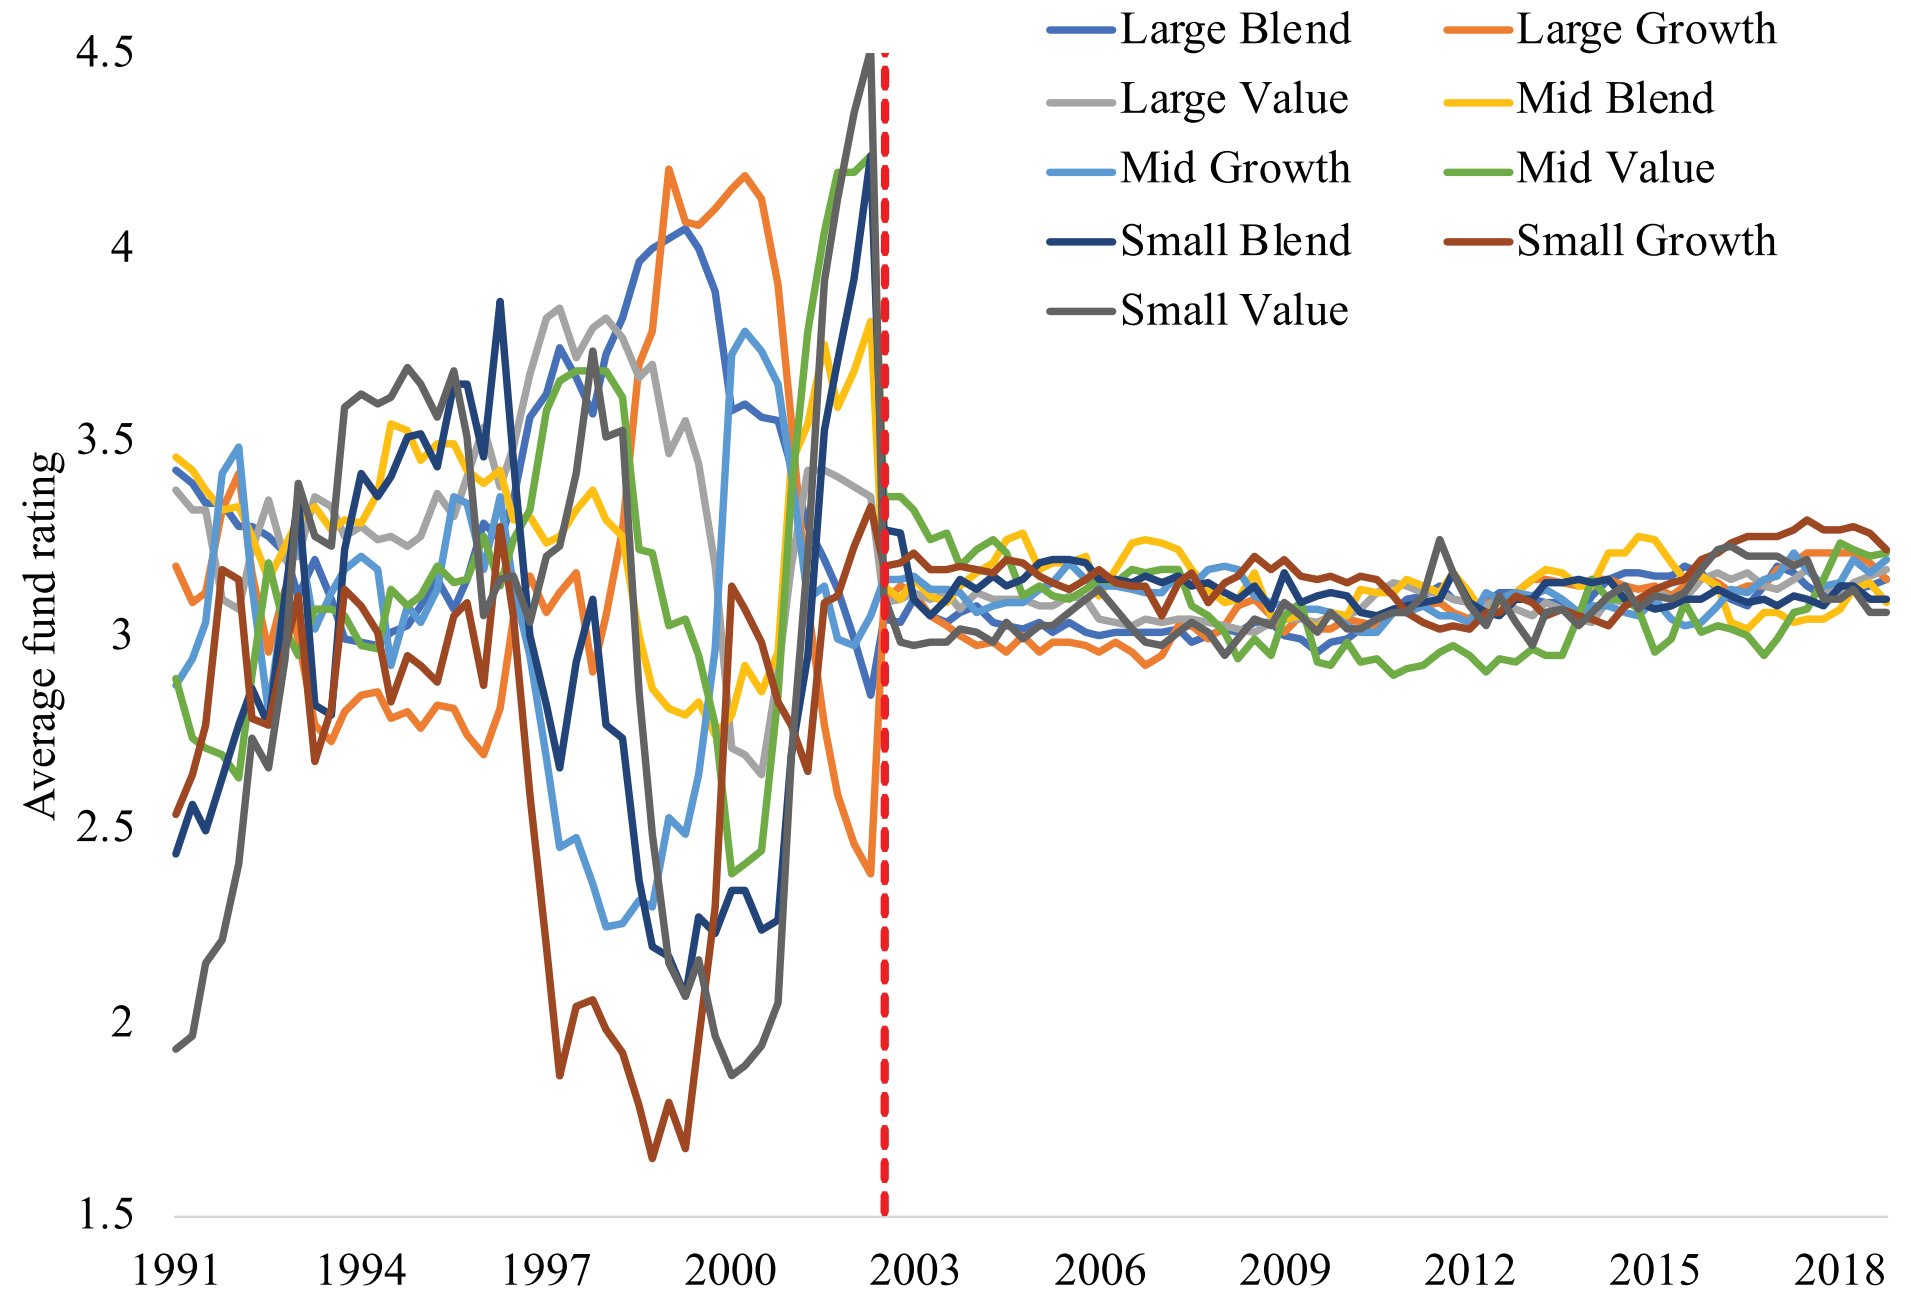
\includegraphics[width=0.85 \linewidth]{pic/fund_rating_by_style.png}
        \end{center}
        \caption{Morningstar fund rating by style}
    \end{figure}
\end{frame}

\section{Data}

\begin{frame}{Variable: Mutual fund sample}
	\begin{itemize}
		\item Monthly fund returns and total net assets from CRSP \\ ( $\mathrm{Ret}_{j, t}$ and $\mathrm{TNA}_{j, t}$ for fund $j$ in month $t$ )
		\item Quarterly fund holdings from Thomson Reuters’ S12
		\item Ratings and style categories from Morningstar Direct
	\end{itemize}
	\\ \ \\
	\ \ \ The \alert{fund flow} is defined as the net flow into the fund divided by lagged TNA:
	$$
	\mathrm{Flow}_{j, t}=\frac{\mathrm{TNA}_{j, t}}{\mathrm{TNA}_{j, t-1}}-\left(1+\mathrm{Ret}_{j, t}\right)
	$$
\end{frame}

\begin{frame}{Variable: Stock- and style-level ratings}
	\alert{Stock}-level ratings:
	$$
	\begin{array}{c}
		\mathrm { Rating }_{i, t}^{\text{stock}}  =\frac{\sum_{\text {fund}\ j \in J} \mathrm{SharesHeld}_{i, j, t-1} \cdot \mathrm{Rating }_{j, t}}{\sum_{\text{fund}\ j\in J} \mathrm{SharesHeld}_{i, j, t-1}}
		\\ \ \\
	 	\Delta\mathrm{Rating}_{i, t}^{\text{stock}} =\frac{\sum_{\mathrm{fund}\ j \in J}\mathrm{SharesHeld}_{i, j, t-1}(\mathrm{Rating}_{j, t}-\text {Rating}_{j, t-1})}{\sum_{\text{fund}\ j\in J} \mathrm{SharesHeld}_{i, j, t-1}}
	 	\end{array}
	$$
	\\ \ \\
	\alert{Style}-level ratings:
	$$
	\begin{array}{c}
	\mathrm{ Rating }_{\pi, t}^{\text{style}}=\sum_{i \in \text{style}\ \pi} w_{i, t-1}^{\pi} \cdot \mathrm{Rating}_{i, t}^{\text{stock}}
	\\ \ \\
	\Delta\mathrm{Rating}_{\pi, t}^{\text{style}}=\sum_{i \in \text{style}\ \pi} w_{i, t-1}^{\pi} \cdot \Delta \mathrm{Rating}_{i, t}^{\text{stock}}
	\end{array}
	$$
	$$
	w_{i, t-1}^{\pi}=\frac{\sum_{\text{fund}\ j \in \text {style}\ \pi } \mathrm{Price}_{i, t-1} \cdot \mathrm{SharesHeld}_{i, j, t-1}}{\sum_{\text{fund}\ j \in \text{style}\ \pi} \mathrm{TNA}_{j, t-1}}
	$$
\end{frame}

\begin{frame}{Exogenous?}
	\begin{itemize}
		\item While the reform was prompted by the dot-com crash and therefore did \alert{not} occur on a random date, its \alert{exact timing} is exogenous
		\item Morningstar \alert{rarely changes} its methodology
		\item The reform is arguably \alert{the most significant change to date}
		\item Investors’ \alert{rating-chasing behavior did not change} around the dot-com bust or the 2002 reform
		\item \alert{Unrelated} to the specific channel of rating-induced flows and price pressures that we are interested in
	\end{itemize}
\end{frame}


\section{Empirical Analysis}

\begin{frame}{How to examine the mechanism?}
	\begin{enumerate}
		\item The key elements of the mechanism exist
		\begin{itemize}
			\item Rating-chasing behavior
			\item Price impact
		\end{itemize}
		\item Rating-driven demand $\rightarrow$ systematic return pattern
		\begin{itemize}
			\item Effects of rating changes on style flows and returns
			\item Examine the rating-driven style momentum strategy
			\item Cross-sectional dispersion in style flows and returns
		\end{itemize}
		\item Event study
		\begin{itemize}
			\item Performance of styles, by predicted rating impact
			\item Placebo test: Other years
			\item Other factors that may have affected style returns
			\item Controlling for stock characteristics
		\end{itemize} 
	\end{enumerate}
\end{frame}

\subsection{Rating-Chasing Behavior and Price Impact}

\begin{frame}{Part \uppercase\expandafter{\romannumeral 1}: Rating-Chasing Behavior and Price Impact}
	 \begin{enumerate}
	 	\item Investors chase ratings regardless of rating methodology
	 	\item Stock-level rating-induced price pressures
	 	\item Return predictability in the cross-section of stock returns
	 \end{enumerate}
\end{frame}

\begin{frame}{Investors chase ratings regardless of rating methodology}
	\begin{figure}[htpb]
	  \begin{center}
	    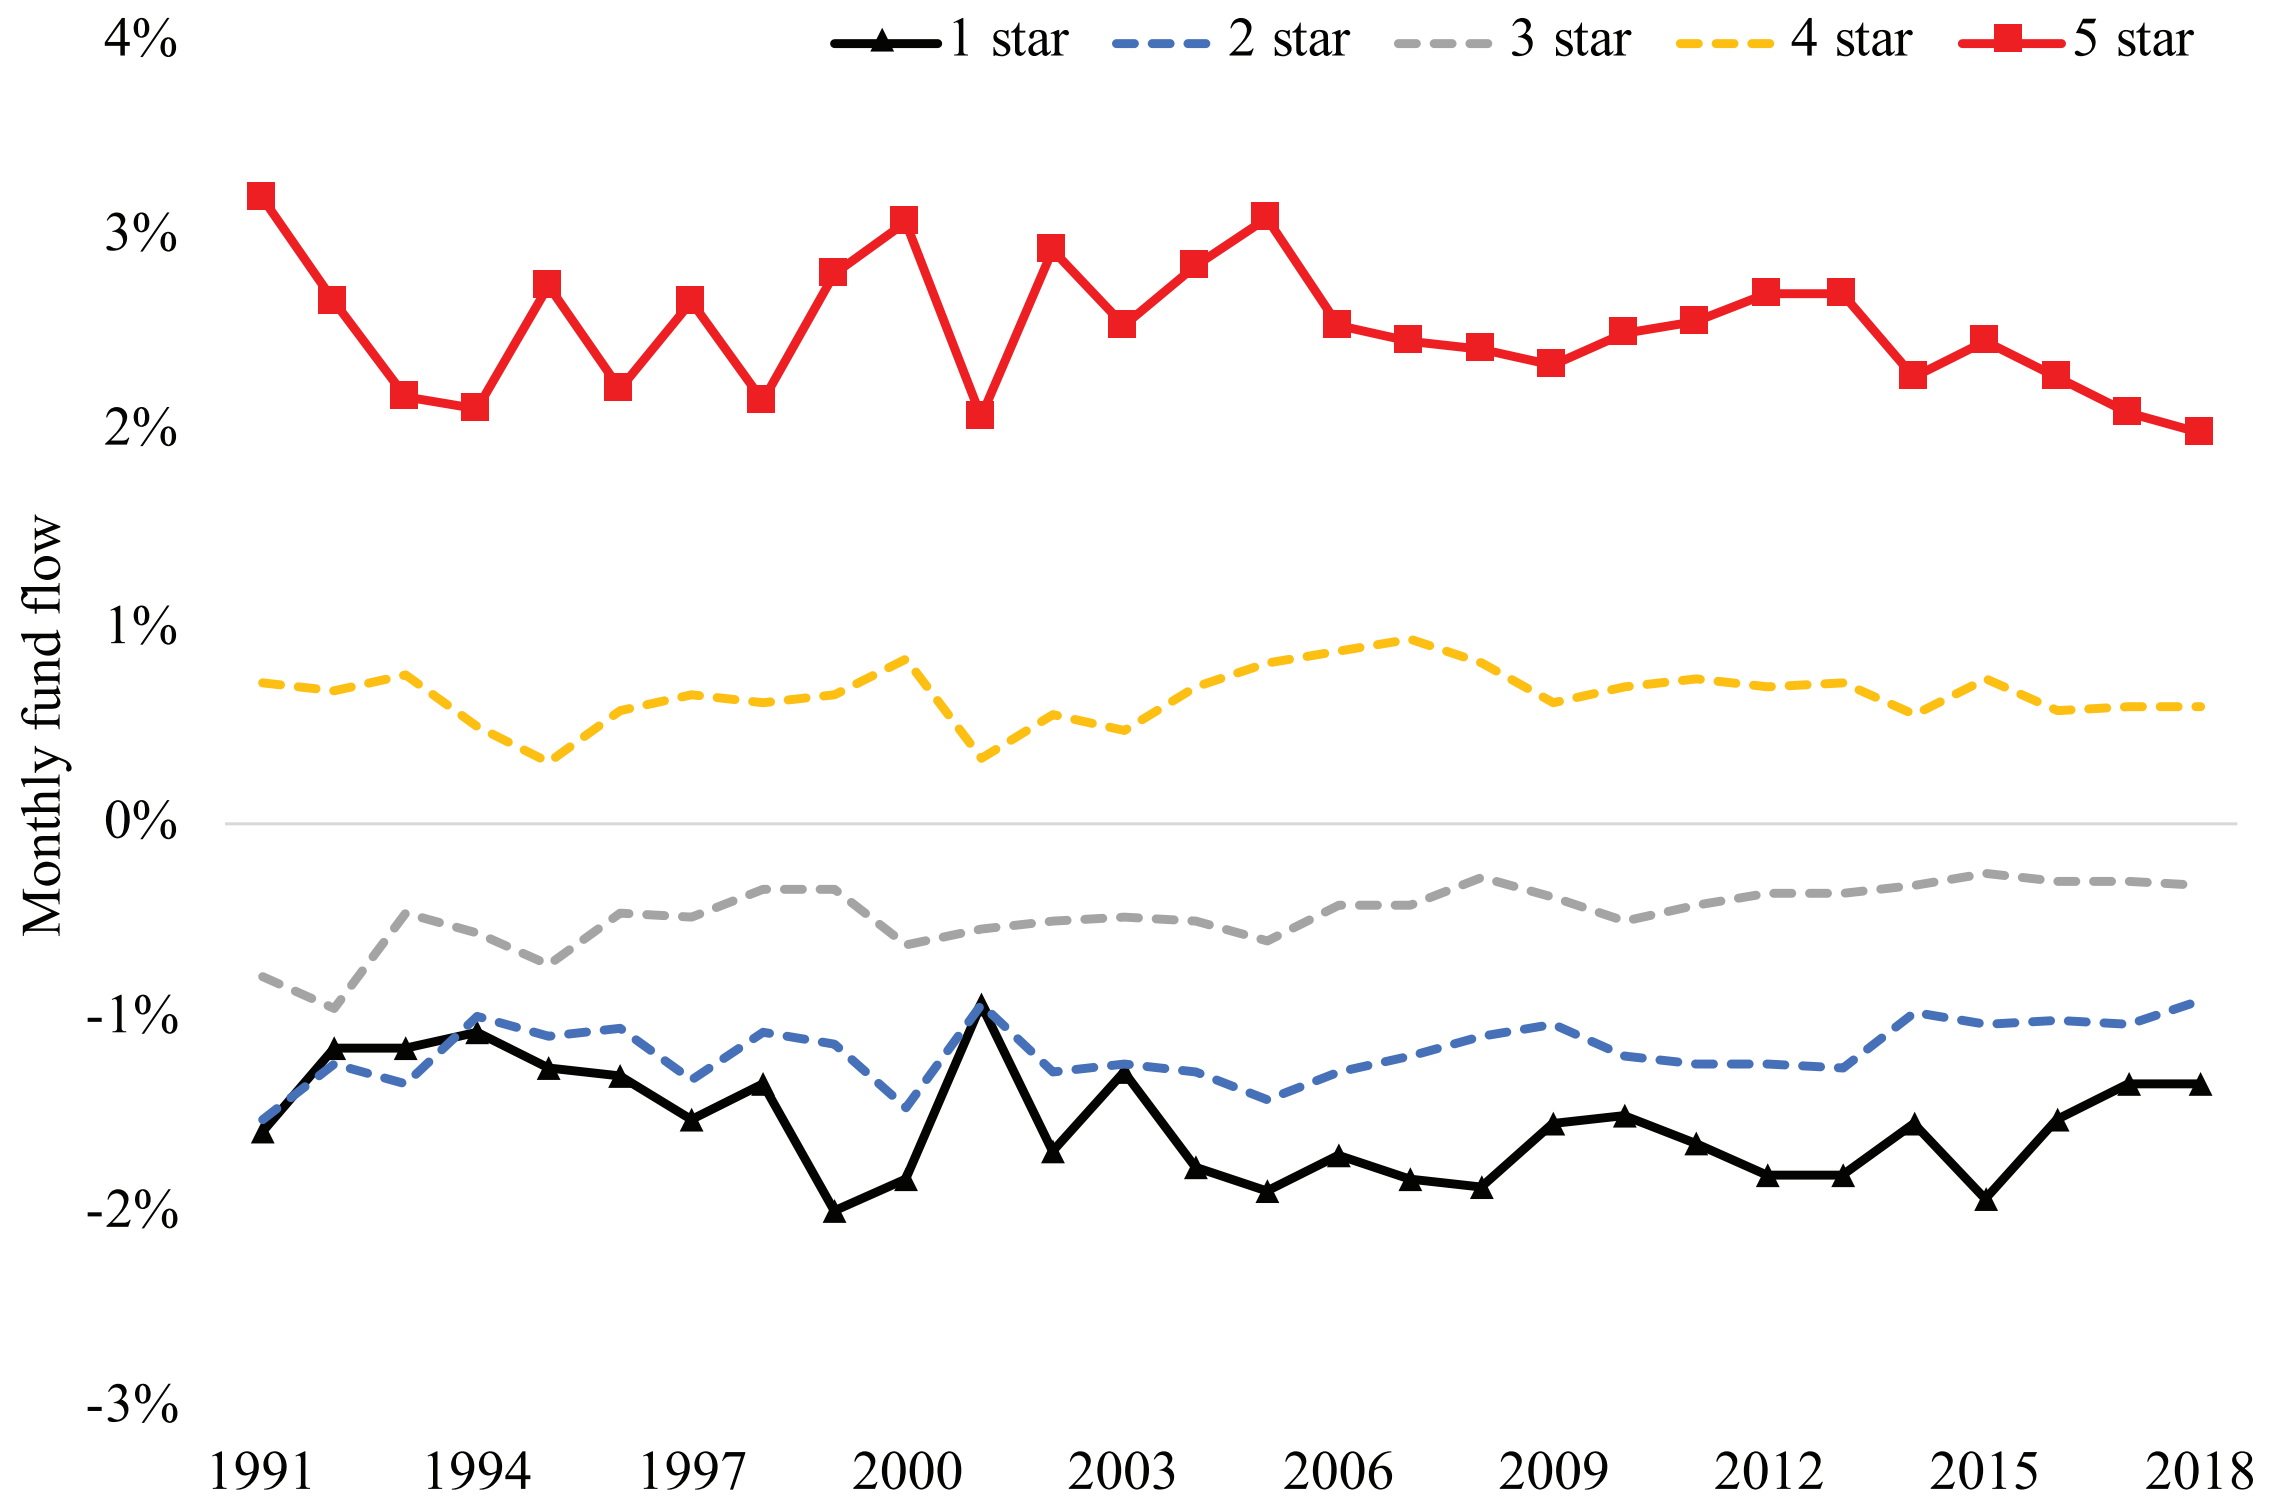
\includegraphics[width=0.85 \linewidth]
	    {pic/fund_flow_by_rating.png}
	  \end{center}
	  \caption{Average flows to mutual funds with different ratings}
	\end{figure}
\end{frame}

\begin{frame}{Investors chase ratings regardless of rating methodology}
	\begin{figure}[htpb]
	  \begin{center}
	    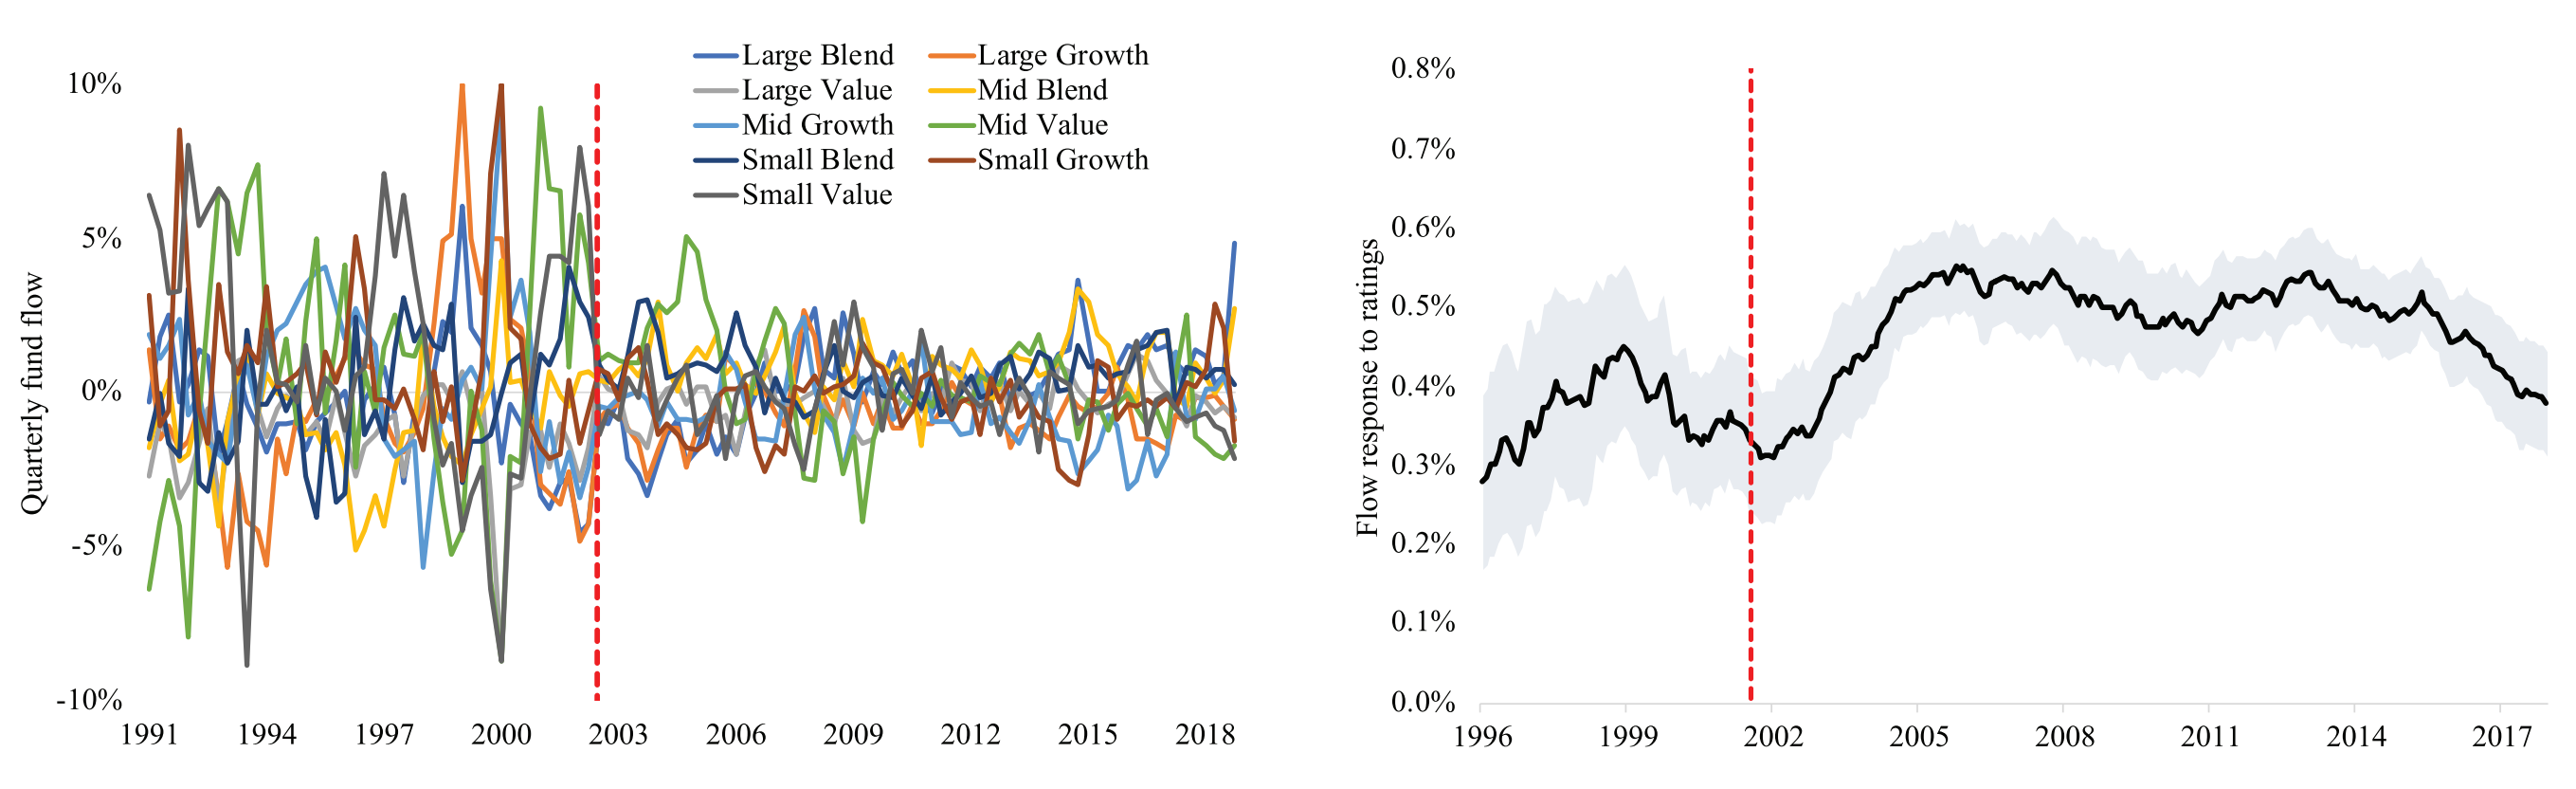
\includegraphics[width=1.06  \linewidth]
	    {pic/fund_flow_change.png}
	  \end{center}
	  \caption{Relation between Morningstar ratings and fund flows}
	\end{figure}
\end{frame}

\begin{frame}{Stock-level rating-induced price pressures}
	\begin{enumerate}
		\item Rating changes $\rightarrow$ Fund flows
		\begin{itemize}
			\item $\mathrm{Flow} _{j, t}=a+b_{1}\Delta\mathrm{Rating}_{j, t-1}+\cdots+b_{36}\Delta\mathrm{Rating}_{j, t-36}+\gamma X_{j, t}+u_{j, t}$
			\item Cumulative response coefficients: $b_1,b_1+b_2,\cdots$
			\item When controlling for past fund performance, discrete changes in ratings cause \alert{sizeable differences in flows}
		\end{itemize}
		\item Flow-induced trading $\rightarrow$ Stock returns
		\begin{itemize}
			\item Flow-induced trading: $\mathrm{FIT}_{i, t}=\frac{\sum_{\text{fund}\ j \in J} \mathrm{SharesHeld}_{i, j, t-1} \cdot \mathrm{Flow}_{j, t}}{\sum_{\text{fund}\ j \in J} \mathrm{SharesHeld}_{i, j, t-1}}$
			\item $\mathrm{Ret}_{i, t}=a+c_{0} \cdot \mathrm{FIT}_{i, t}+c_{1} \cdot \mathrm{FIT}_{i, t-1}+\ldots+c_{36} \cdot \mathrm{FIT}_{i, t-36}+u_{i, t}$
			\item Cumulative response: $c_0,c_0+c_1,\cdots$
			\item \alert{Immediate price pressure} in the contemporaneous month and \alert{a complete reversion} in the subsequent 1 to 2 years
		\end{itemize}
	\end{enumerate}
\end{frame}

\begin{frame}{Stock-level rating-induced price pressures}
	\begin{figure}[htpb]
	  \begin{center}
	    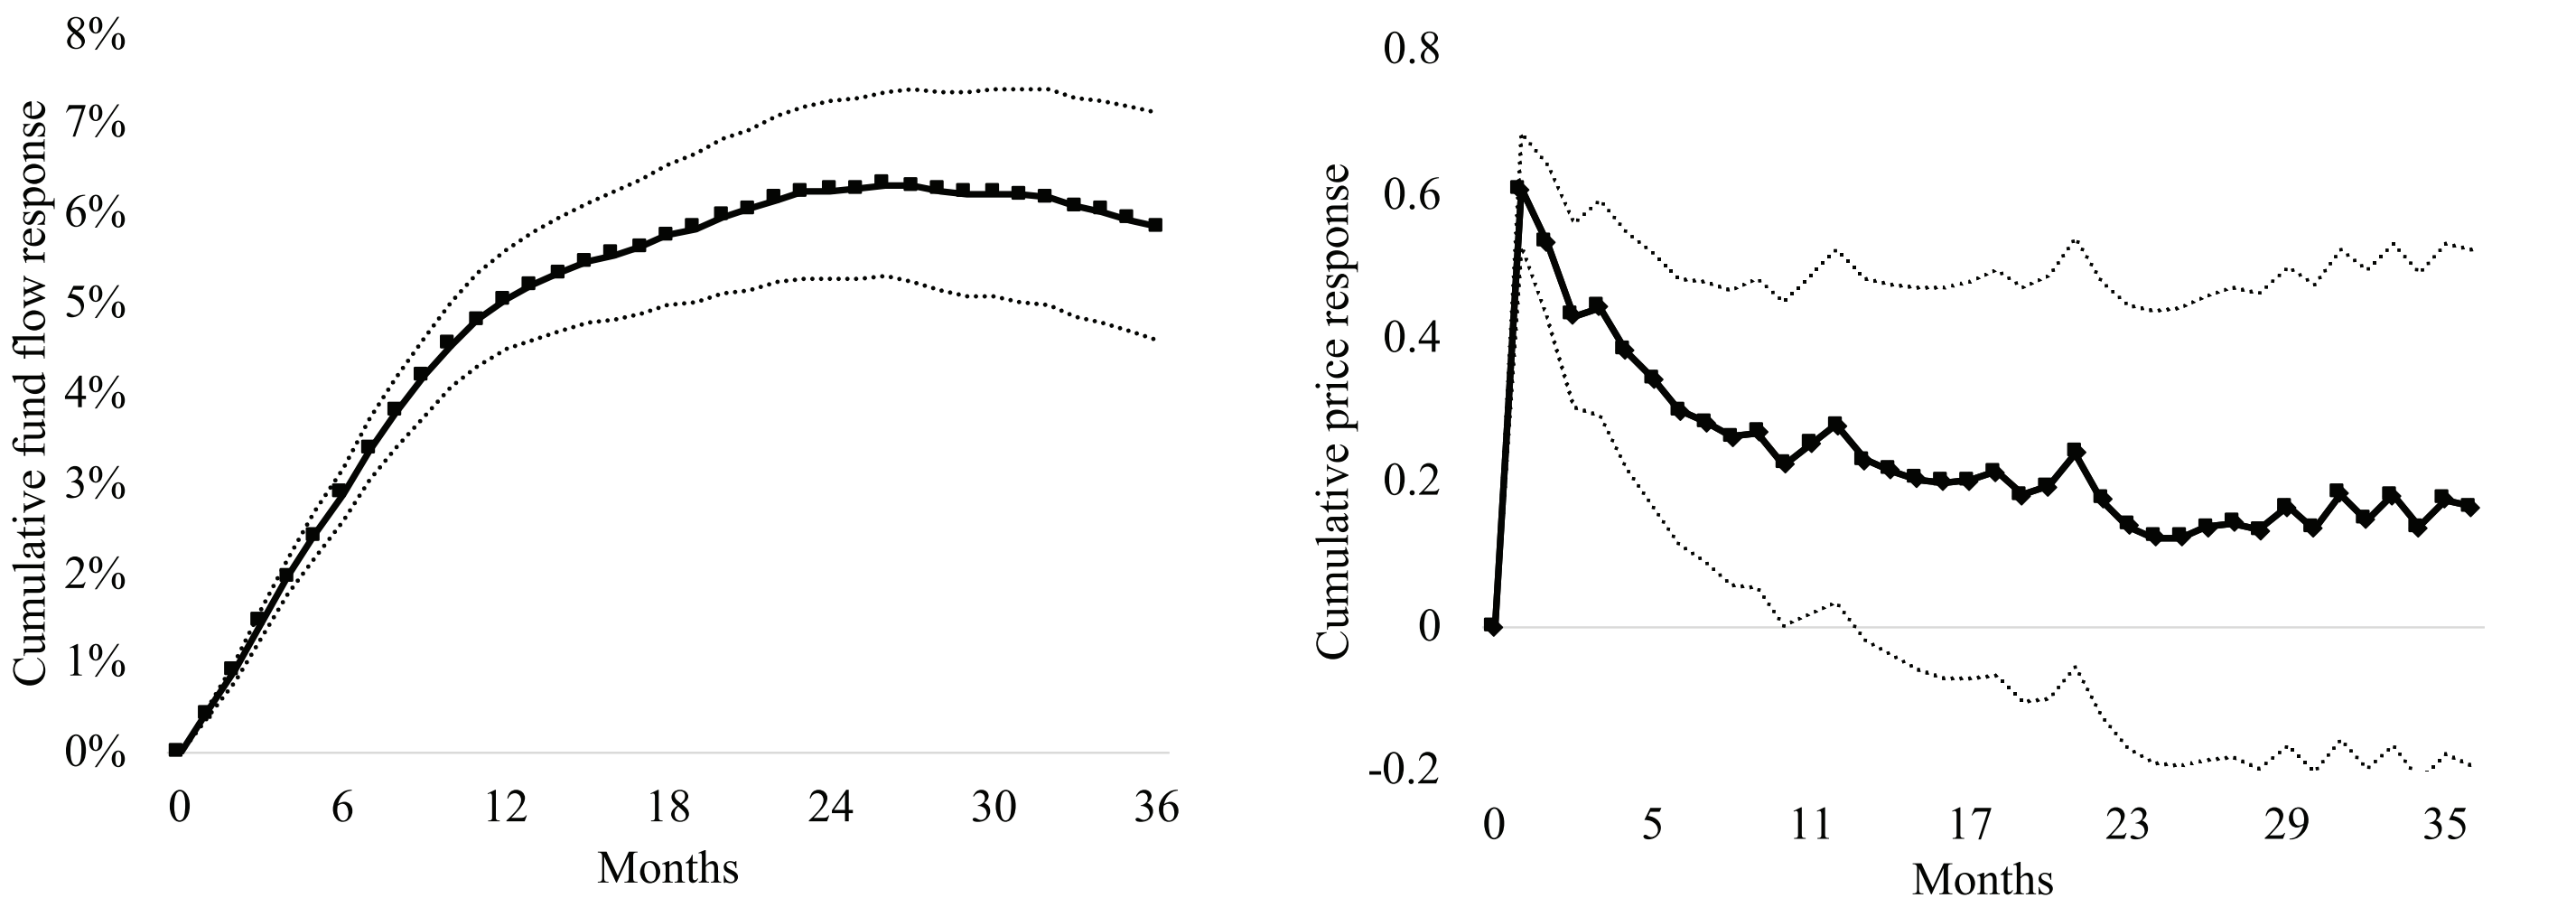
\includegraphics[width=1.06  \linewidth]
	    {pic/price_impact.png}
	  \end{center}
	  \caption{Rating changes, flow-induced trading and returns}
	\end{figure}
\end{frame}

\begin{frame}{Stock-level rating-induced price pressures}
	\begin{itemize}
		\item Estimate the response of stock returns on the past 24 lags of stock-level rating changes
		\item Summarize past rating changes using $\mathrm{ExpSum}(\Delta\mathrm{Rating})_{i, t-1}=\sum_{k=1}^{12} \tau_{k} \cdot \Delta \mathrm{Rating}_{i, t-k}$, where $\tau_{k}=\frac{12 \cdot(1-\delta)}{1-\delta^{12}} \cdot \delta^{k-1}$ and $\delta=0.76$
	\end{itemize}
	\begin{figure}[htpb]
	  \begin{center}
	    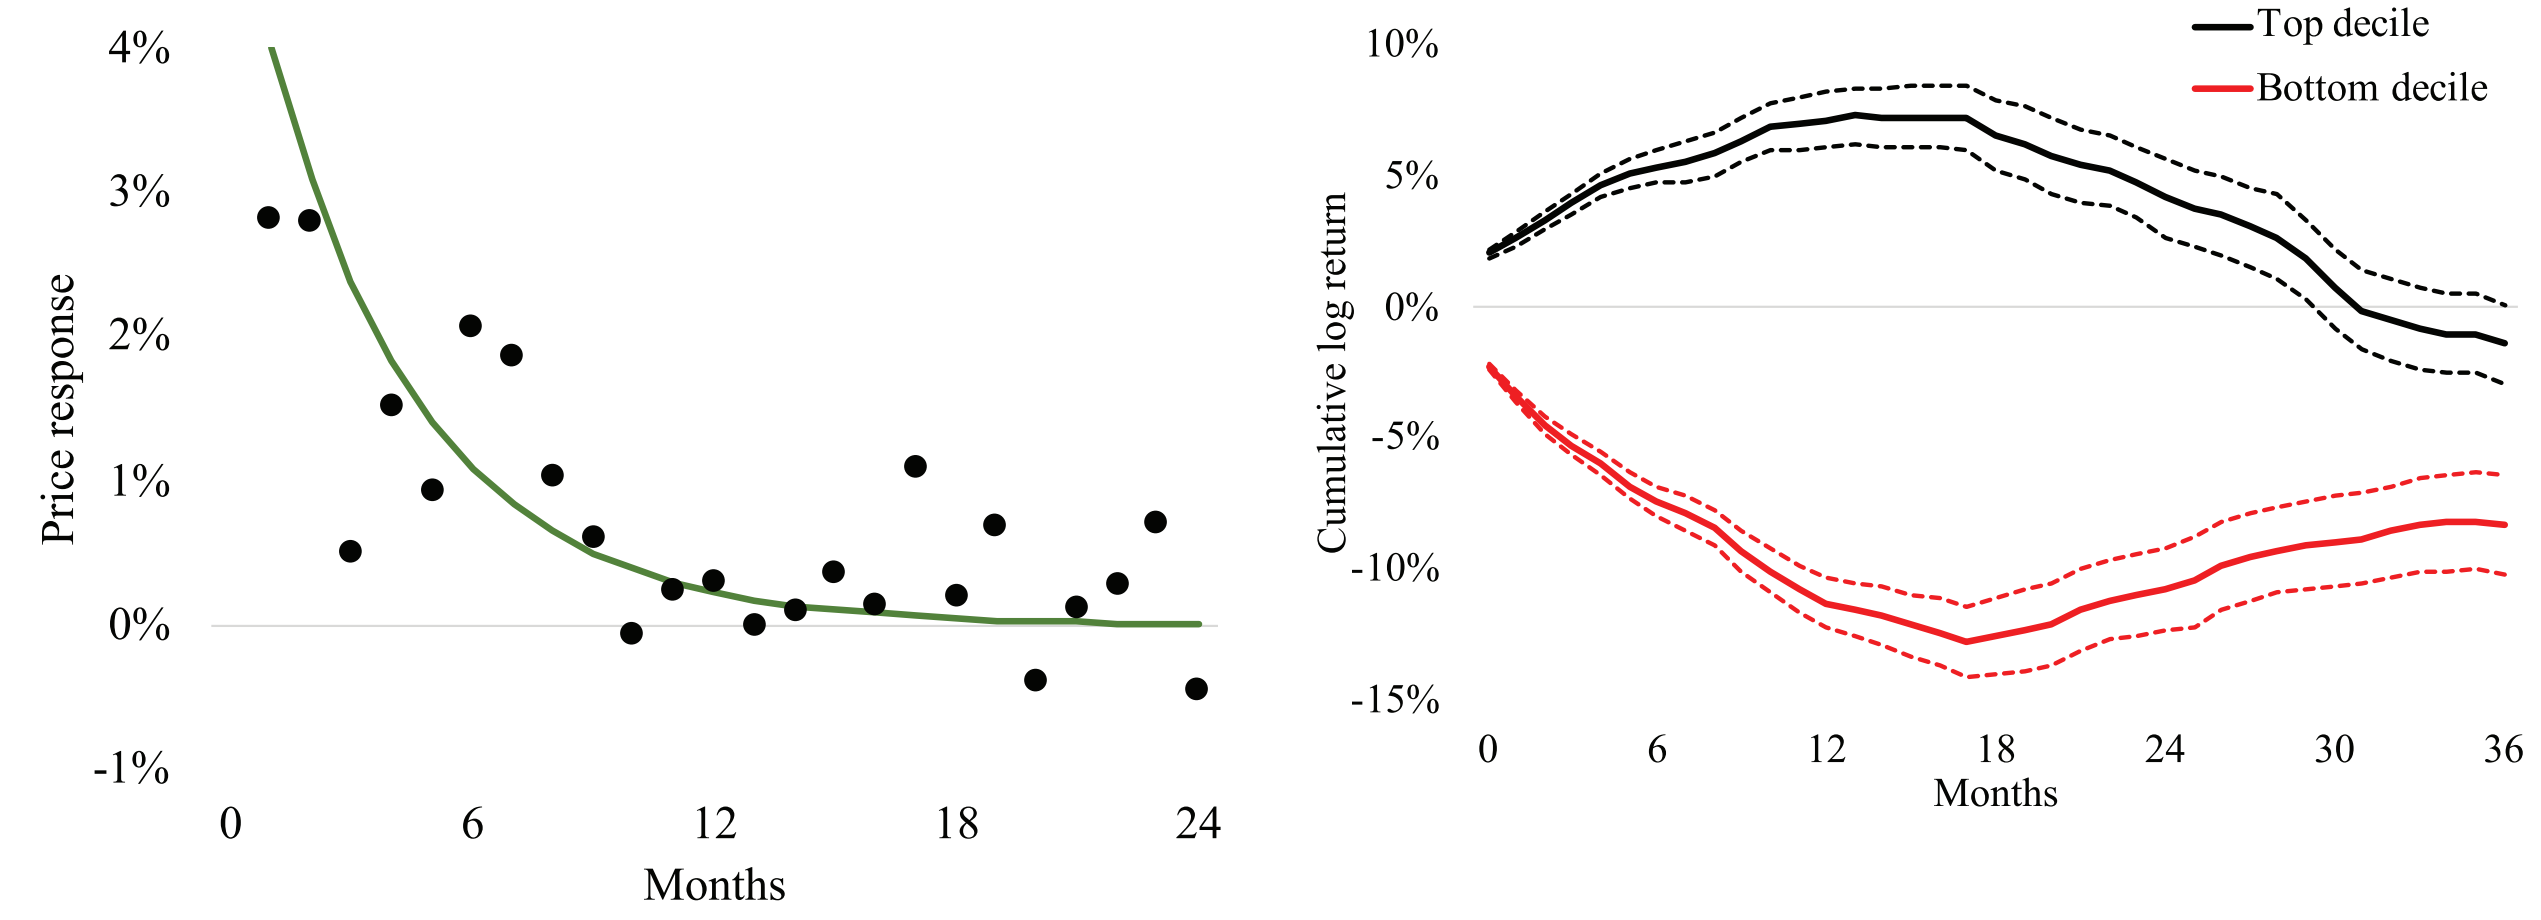
\includegraphics[width=0.89  \linewidth]
	    {pic/rating_changes_return.png}
	  \end{center}
	  \caption{rating changes $\rightarrow$ stock return}
	\end{figure}
\end{frame}

\begin{frame}{Return predictability in the cross-section of stock returns}
	\vspace{-0.6cm}
	$$\mathrm{Return}_{i, t}=d_{1} \Delta \mathrm{Rating}_{i, t-1-h \rightarrow t-1}+\gamma^{s} X_{i, t}^{s}+\gamma^{f} X_{i, t}^{f}+u_{i, t}$$
	\center \tiny{Return predictability from ratings and stock characteristics}
	\vspace{-0.3cm}
	\begin{figure}[htpb]
	  \begin{center}
	    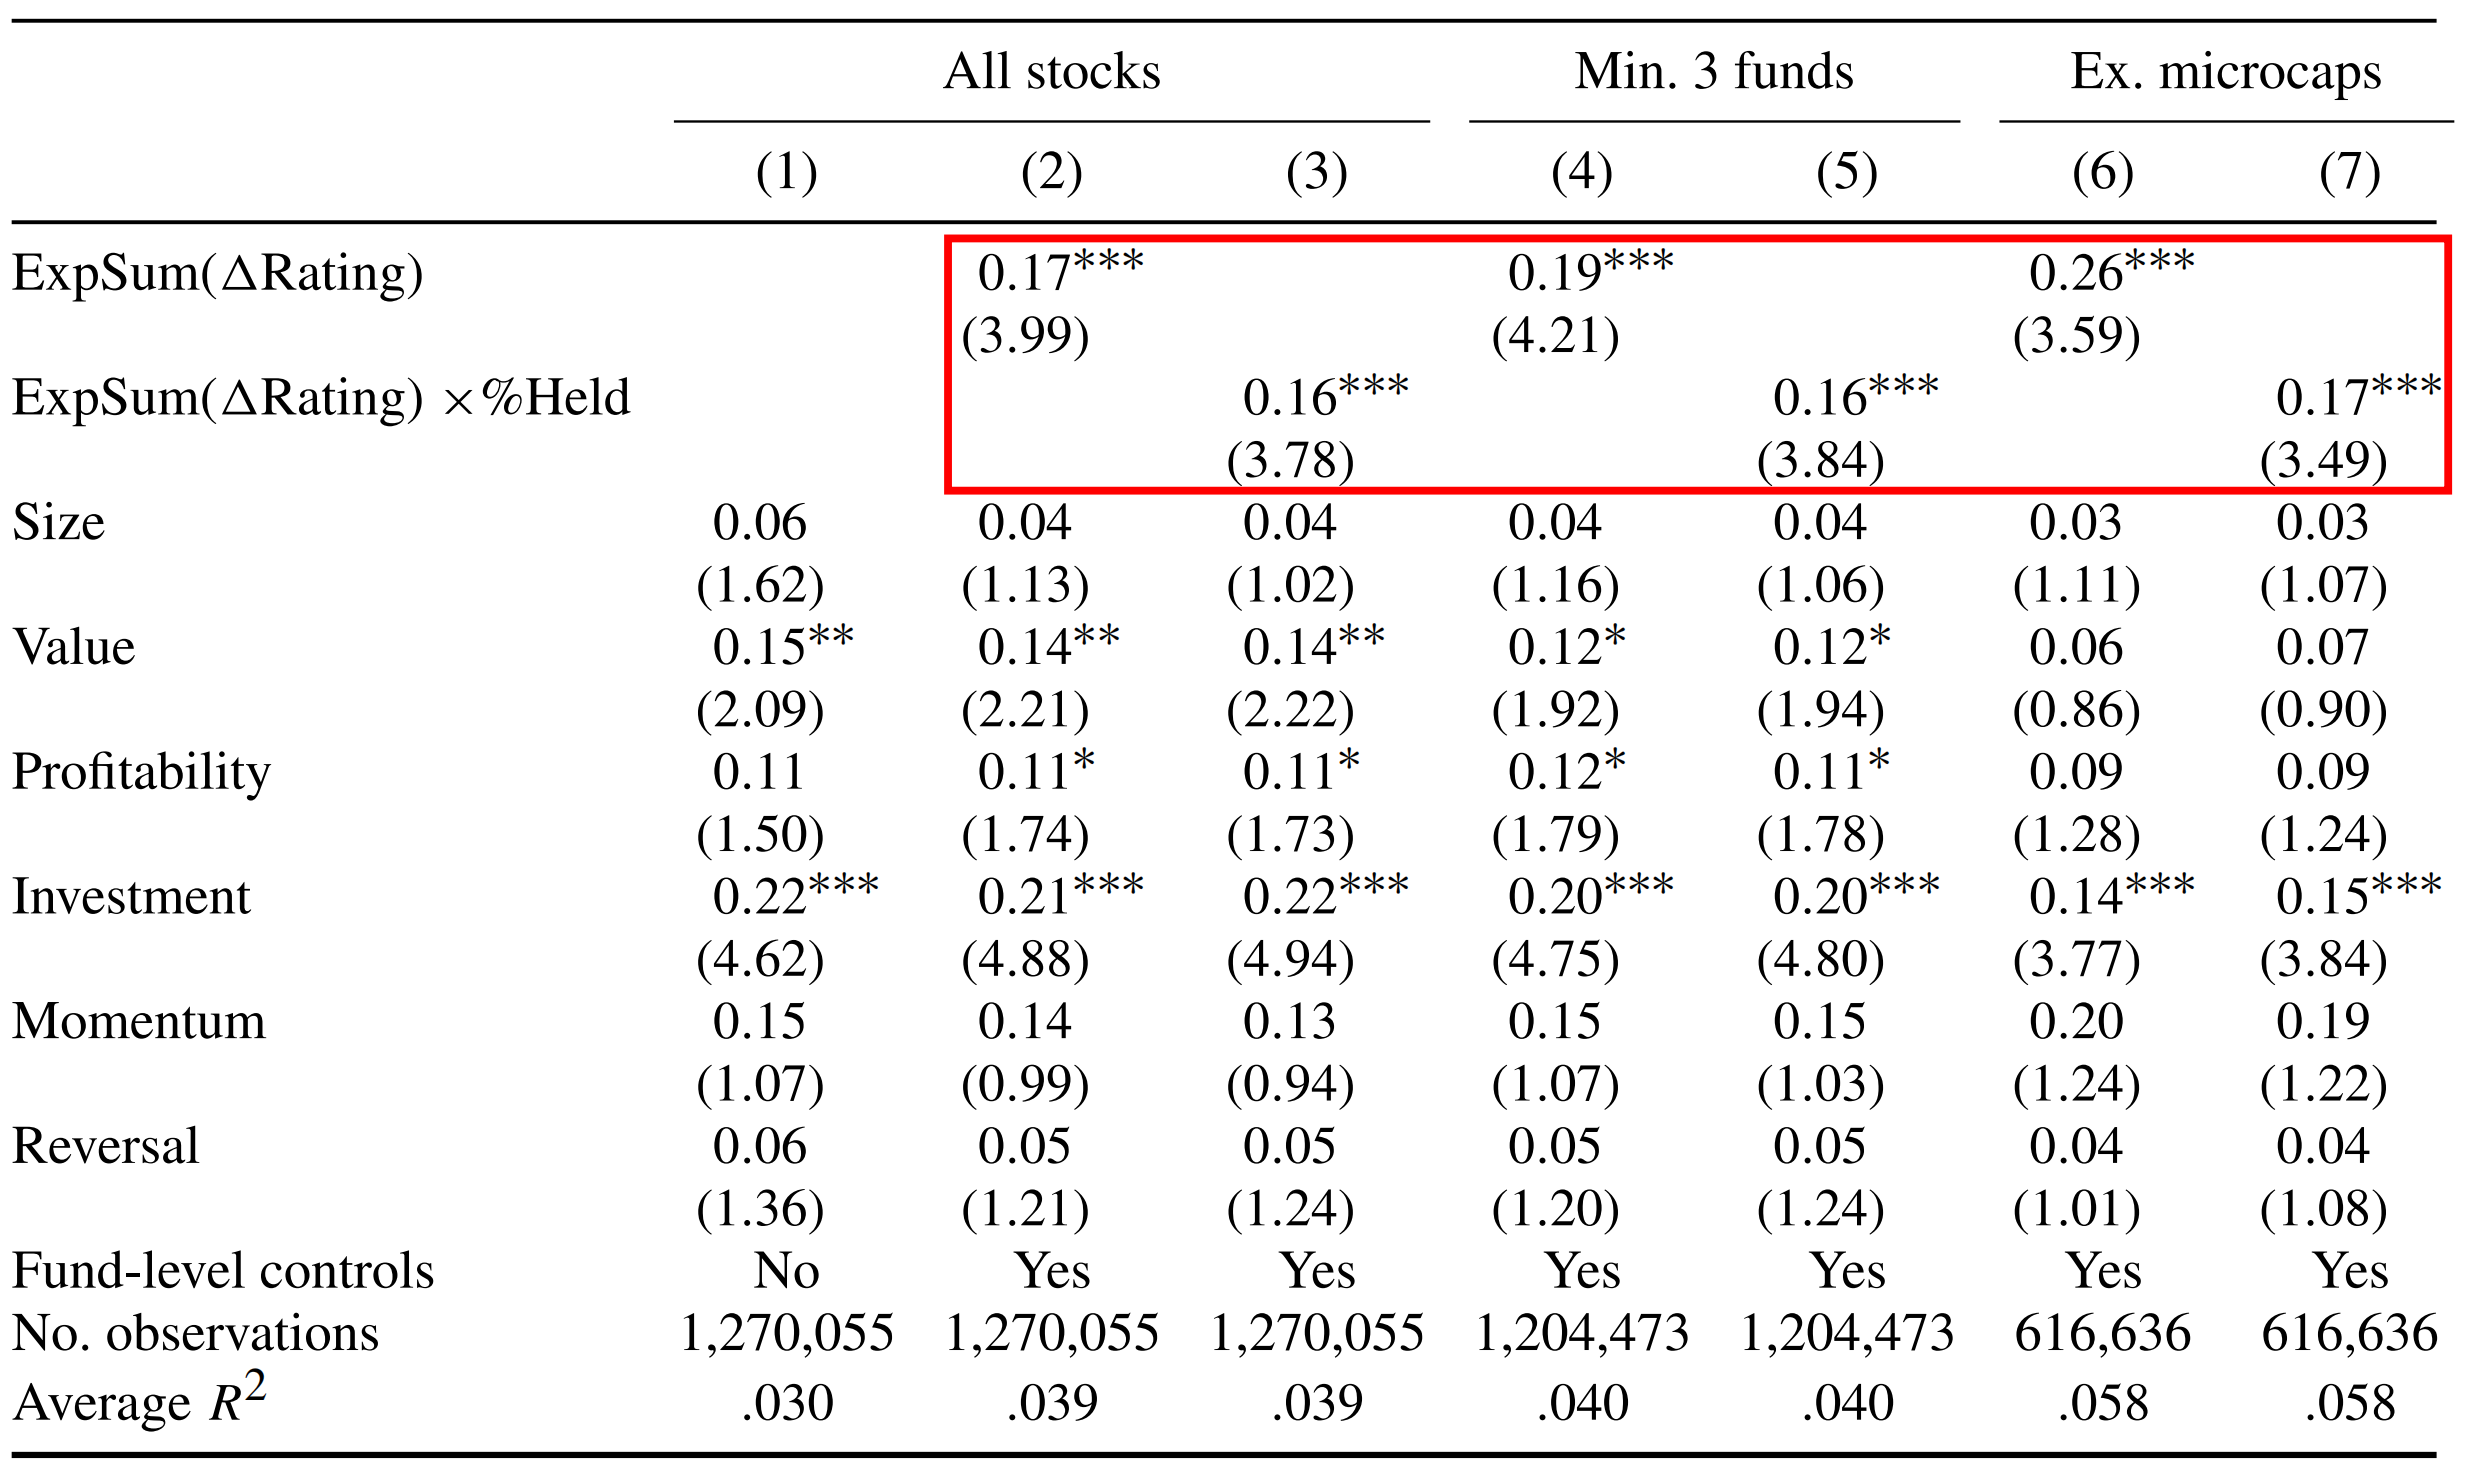
\includegraphics[width=0.89  \linewidth]
	    {pic/return_predictability.png}
	  \end{center}
	\end{figure}
\end{frame}

\subsection{Impact of Rating-Chasing Demand on Style Performance}

\begin{frame}{Part \uppercase\expandafter{\romannumeral 2}: Impact of Rating-Chasing Demand on Style Performance}
	 \begin{enumerate}
	 	\item \alert{Style-level} rating-induced price pressures
	 	\item Rating-driven \alert{style} momentum strategy
	 	\item Cross-sectional dispersion in \alert{style} flows and returns
	 \end{enumerate}
\end{frame}

\begin{frame}{Style-level rating-induced price pressures}
	Style-level changes in Morningstar ratings:
	$$
	\mathrm{ExpSum}(\Delta \mathrm{Rating})_{\pi, t-1}=\sum_{ {i\in\pi}}{w_{i, t-1}^{\pi}} \cdot \mathrm{ExpSum}(\Delta \mathrm{Rating})_{i, t-1}
	$$
	\center \tiny{Rating-induced price pressures in style portfolios}
	\vspace{-0.3cm}
	\begin{figure}[htpb]
	  \begin{center}
	    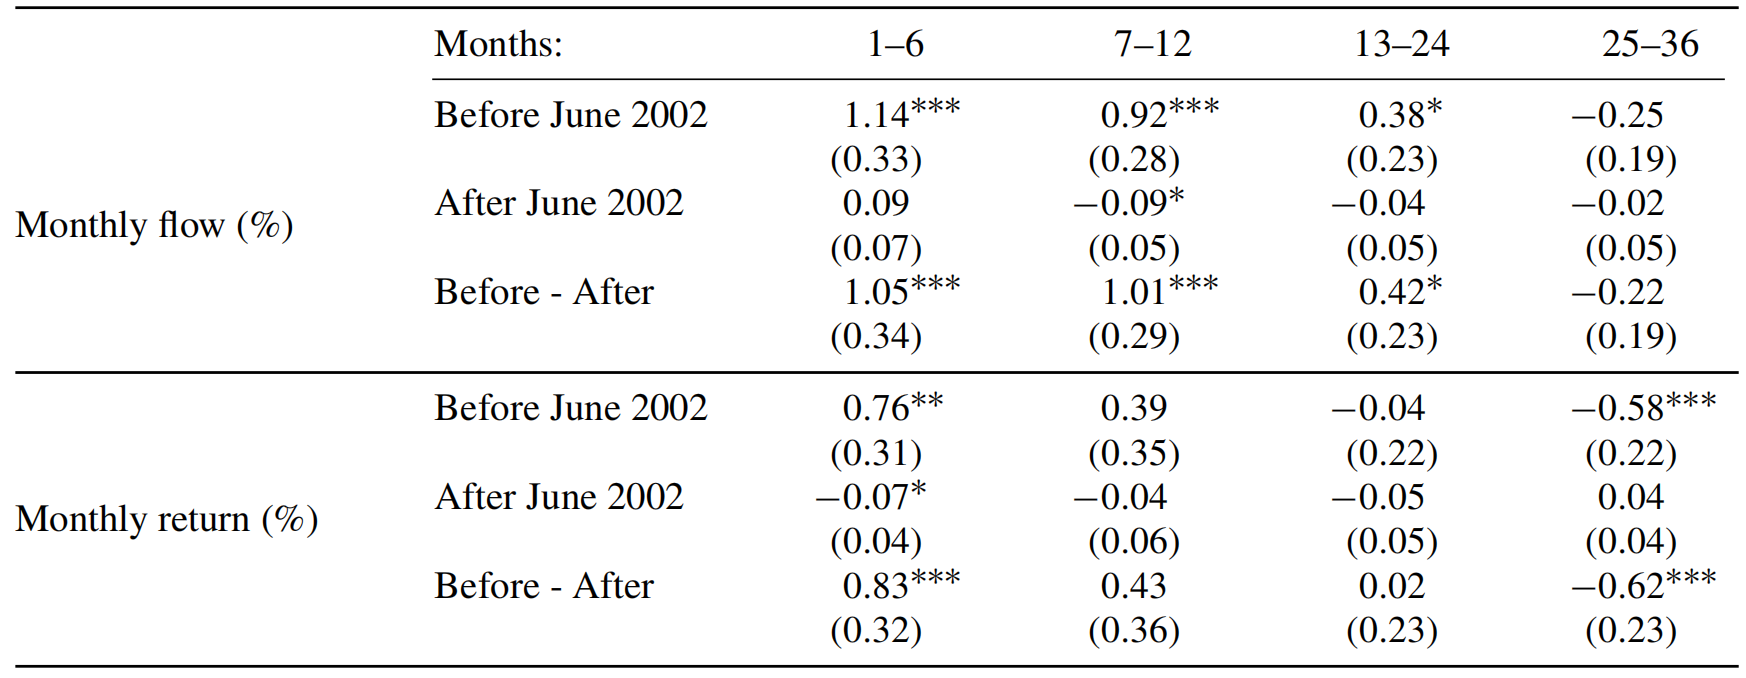
\includegraphics[width=1  \linewidth]
	    {pic/style_portfolios.png}
	  \end{center}
	\end{figure}
\end{frame}

\begin{frame}{Profitability of the rating-driven style momentum strategy}
	\begin{itemize}
		\item A rating-based style momentum strategy would be \alert{profitable} before June 2002, but not afterward
	\end{itemize}
	\center\tiny{Rating-induced style momentum strategy before and after June 2002}
	\vspace{-0.3cm}
	\begin{figure}[htpb]
	  \begin{center}
	    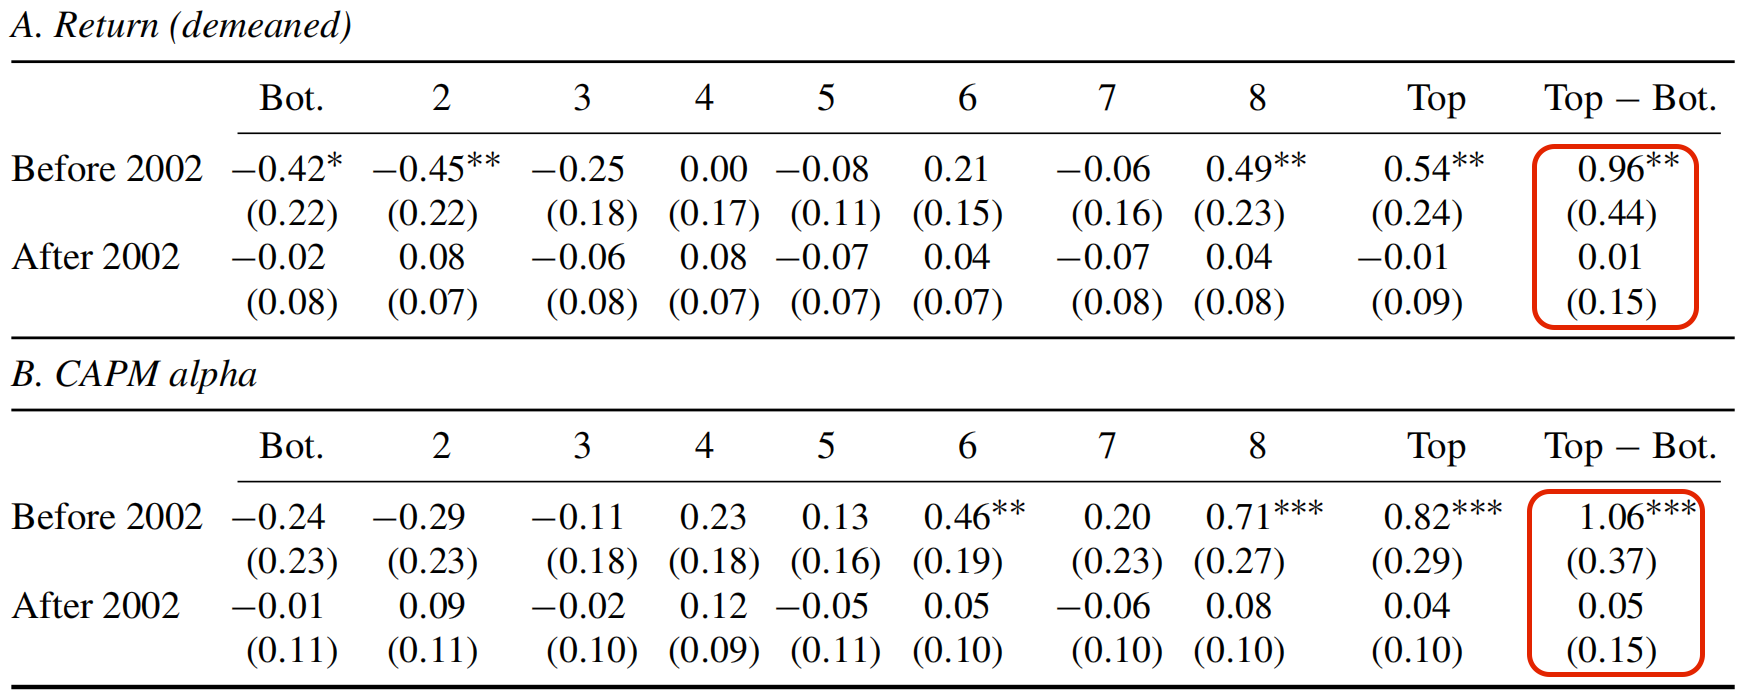
\includegraphics[width=1  \linewidth]
	    {pic/style_momentum_strategy.png}
	  \end{center}
	\end{figure}
\end{frame}

\begin{frame}{Cross-sectional dispersion in style flows and returns}
	If ``ratings drive flows and then lead to price impact" is correct, we should observe \alert{a decline in the dispersion} in style flows and returns after the reform
	\center\tiny{Dispersion of style ratings, flows, and returns}
	\vspace{-0.3cm}
	\begin{figure}[htpb]
	  \begin{center}
	    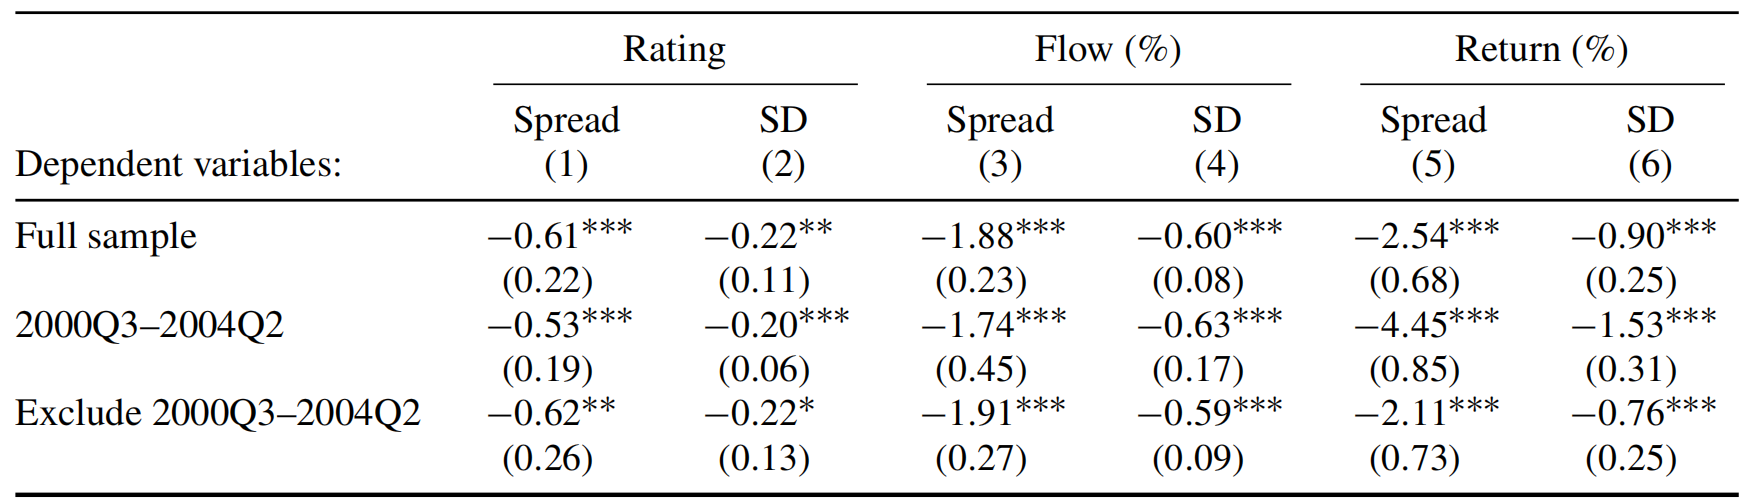
\includegraphics[width=1  \linewidth]
	    {pic/dispersion.png}
	  \end{center}
	\end{figure}
\end{frame}

\subsection{Event Study around the Morningstar Reform}

\begin{frame}{Part \uppercase\expandafter{\romannumeral 3}: Event study}
	\begin{enumerate}
		\item Performance of styles, by predicted rating impact
		\item Placebo test: Other years
		\item Other factors that may have affected style returns
		\item Controlling for stock characteristics
	\end{enumerate}
\end{frame}

\begin{frame}{Performance of styles, by predicted rating impact}
	\begin{itemize}
		\item An additional and independent test of rating-induced demand effects on style returns
		\item Ensure that the rating changes are \alert{primarily caused by the methodology change}
		\item Reduces the chance that our findings are confounded by \alert{other events}
	\end{itemize}
	\begin{columns}
		\column{0.33\textwidth}
		\begin{figure}[htpb]
		  \begin{center}
		    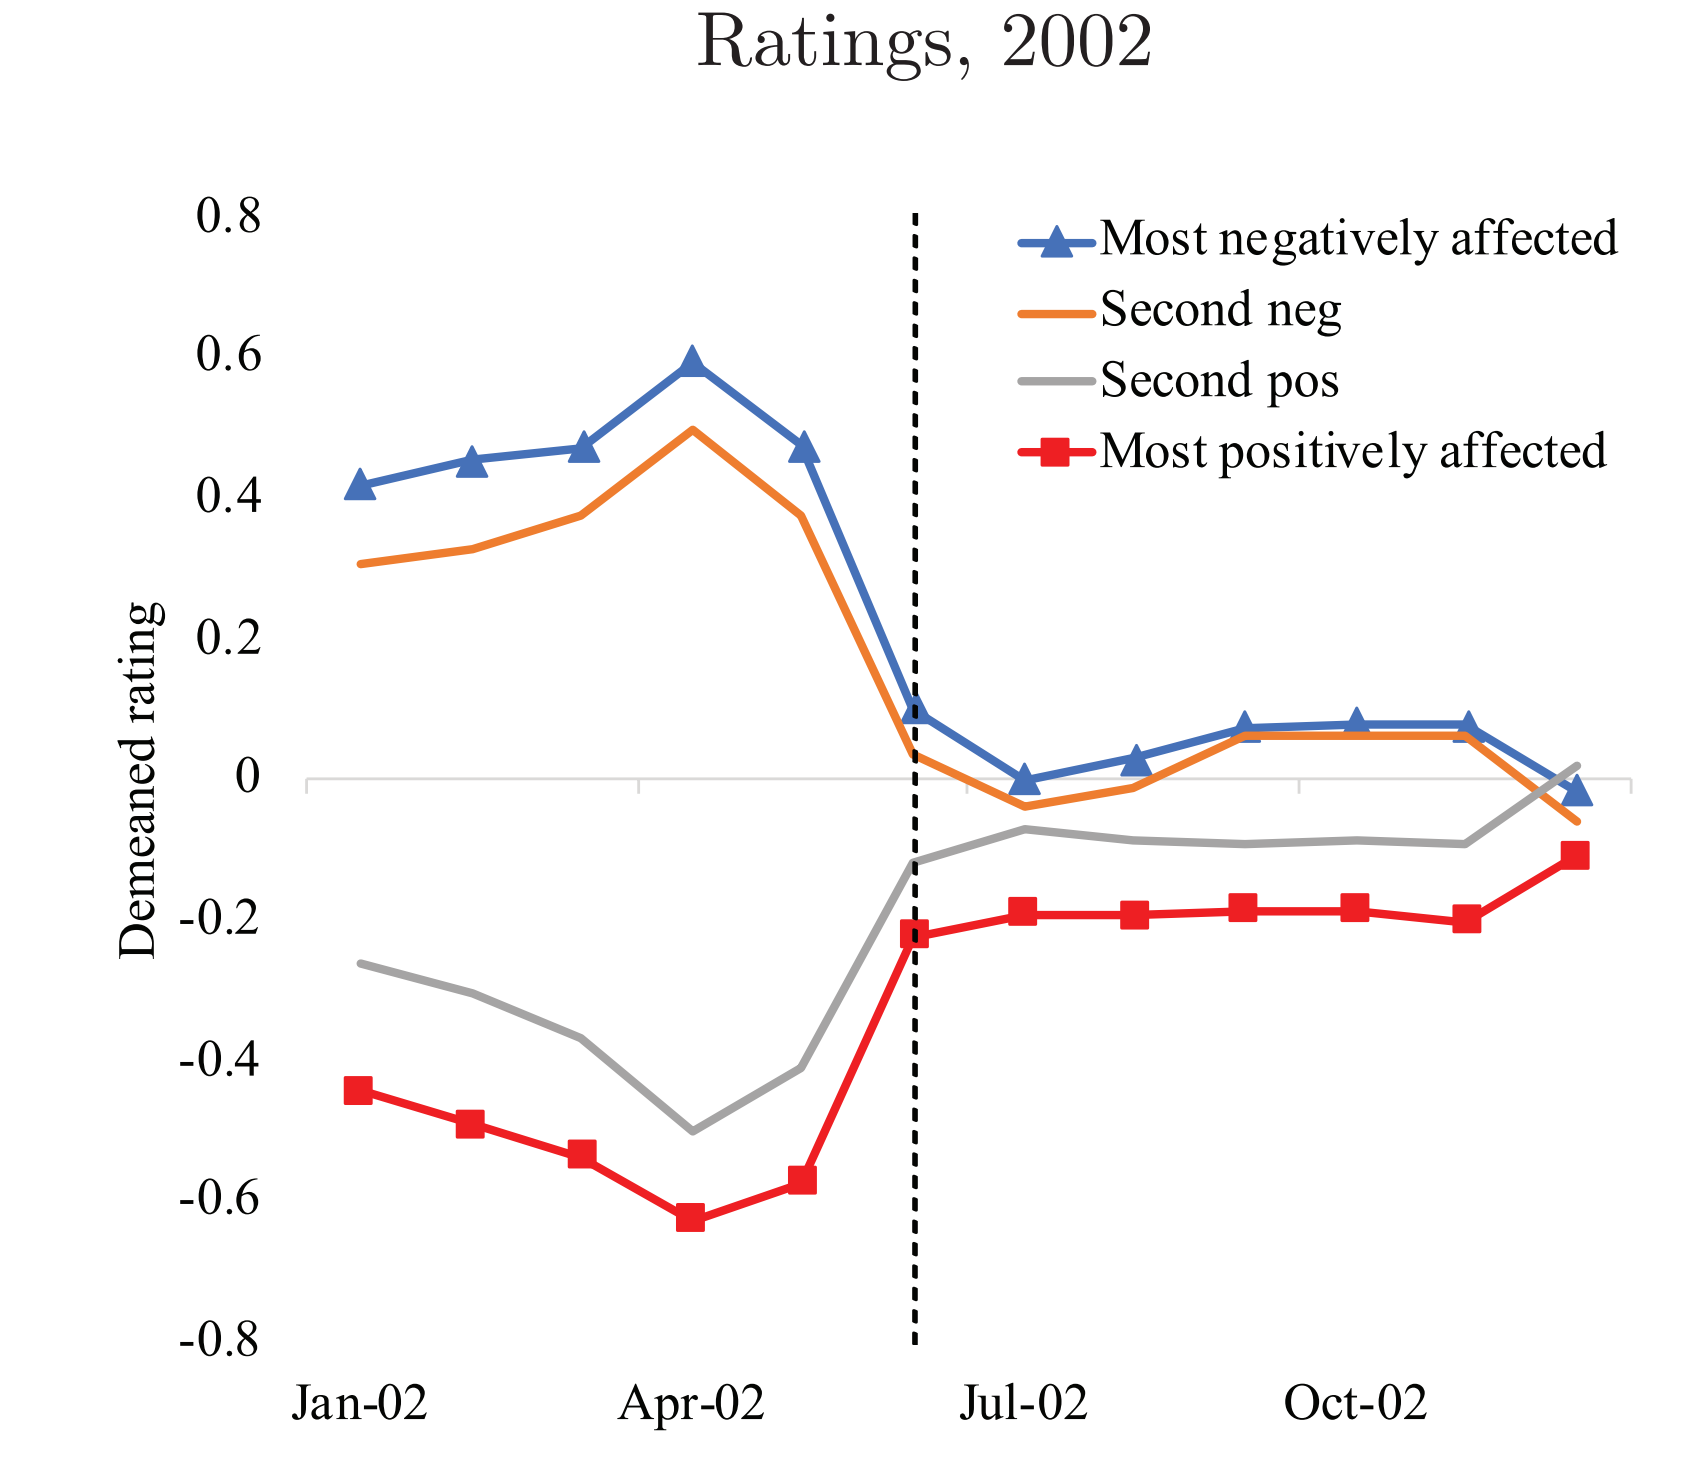
\includegraphics[width=1  \linewidth]
		    {pic/event_ratings.png}
		  \end{center}
		\end{figure}
		\vspace{-0.6cm}
		\center\tiny{Average style ratings}
		\column{0.33\textwidth}
		\begin{figure}[htpb]
		  \begin{center}
		    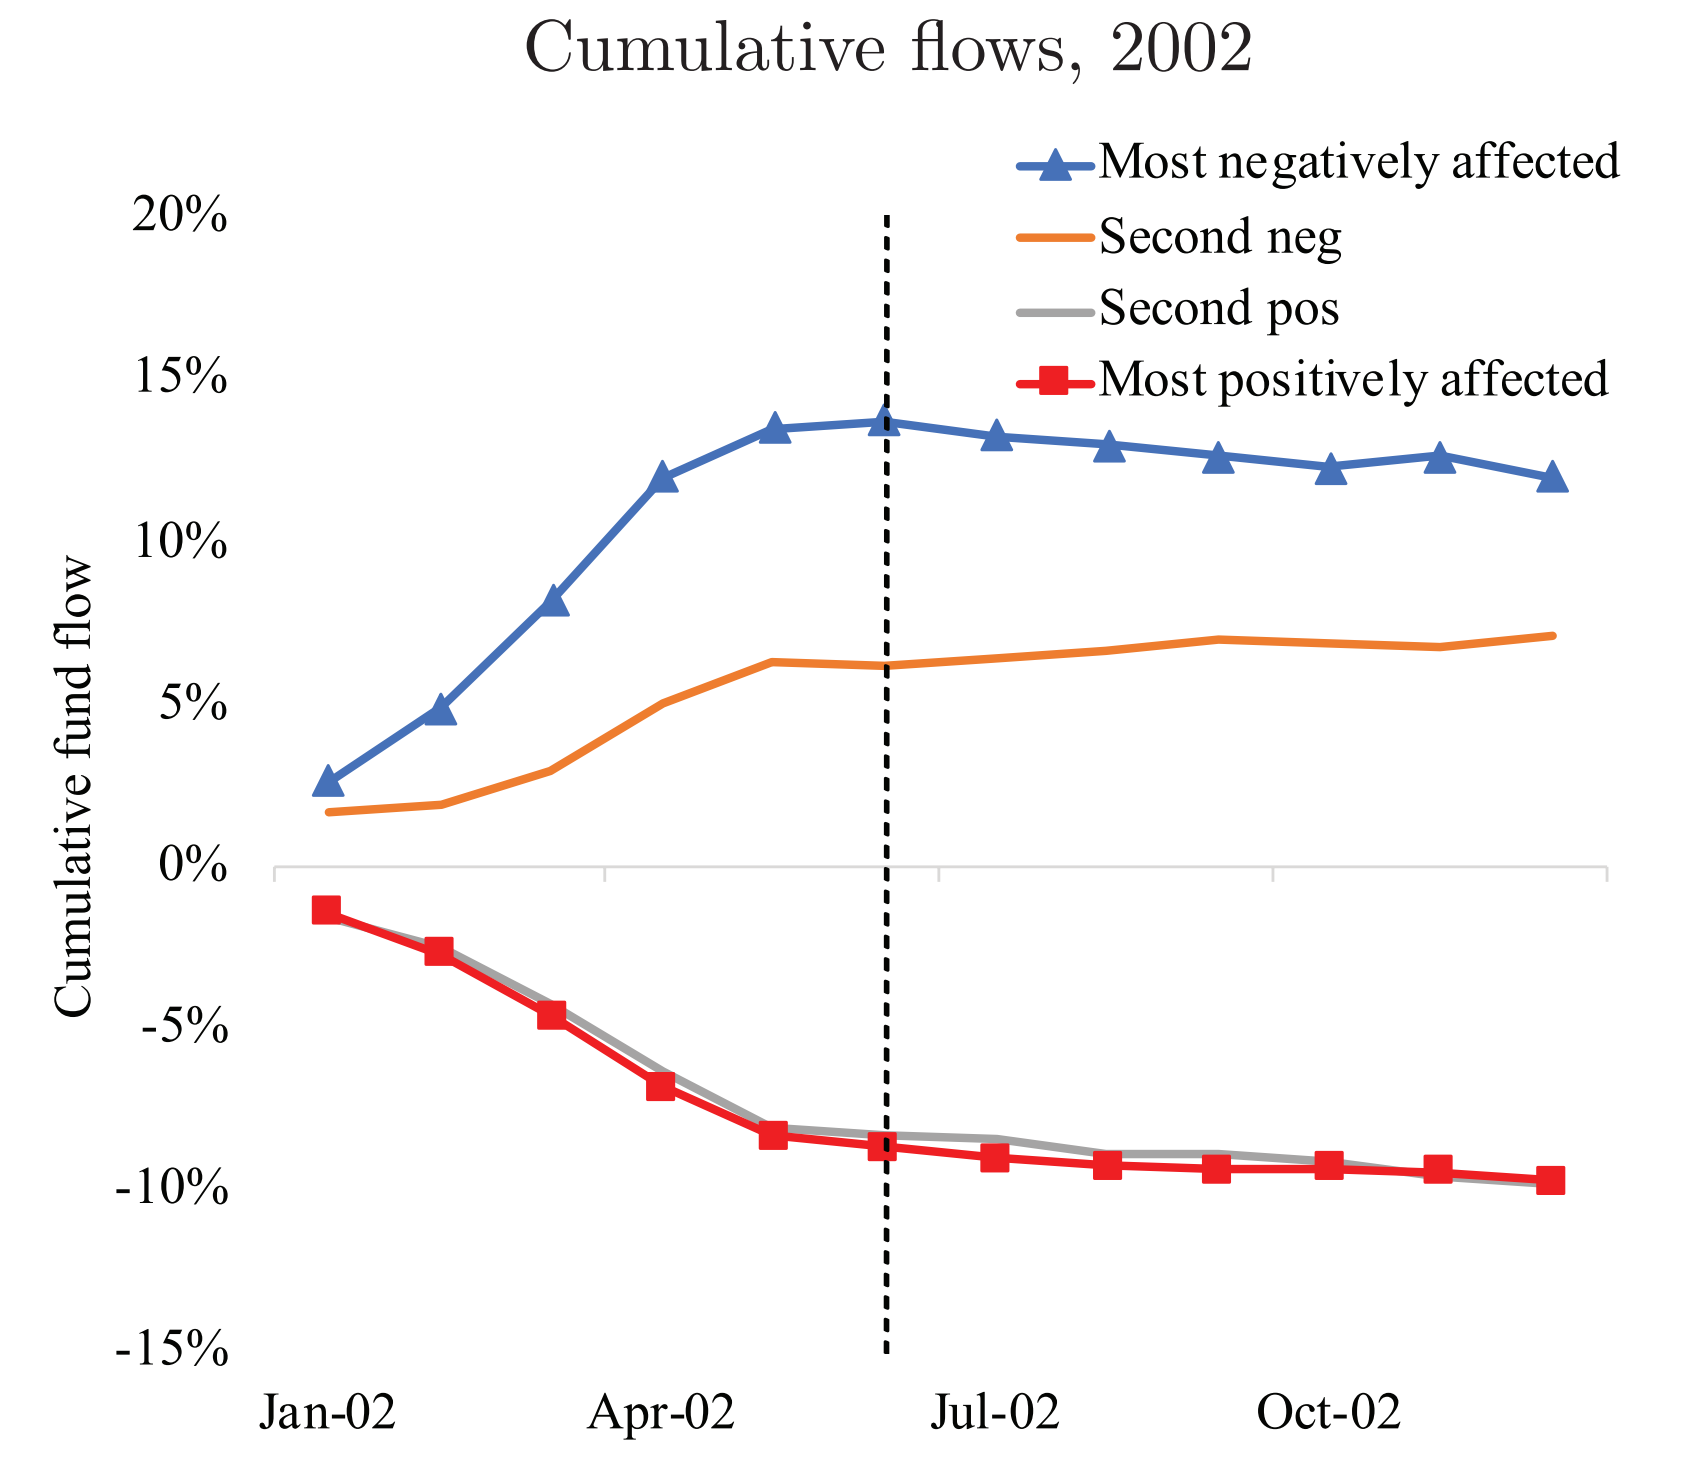
\includegraphics[width=1  \linewidth]
		    {pic/event_flows.png}
		  \end{center}
		\end{figure}
		\vspace{-0.6cm}
		\center\tiny{Cumulative style flows}
		\column{0.33\textwidth}
		\begin{figure}[htpb]
		  \begin{center}
		    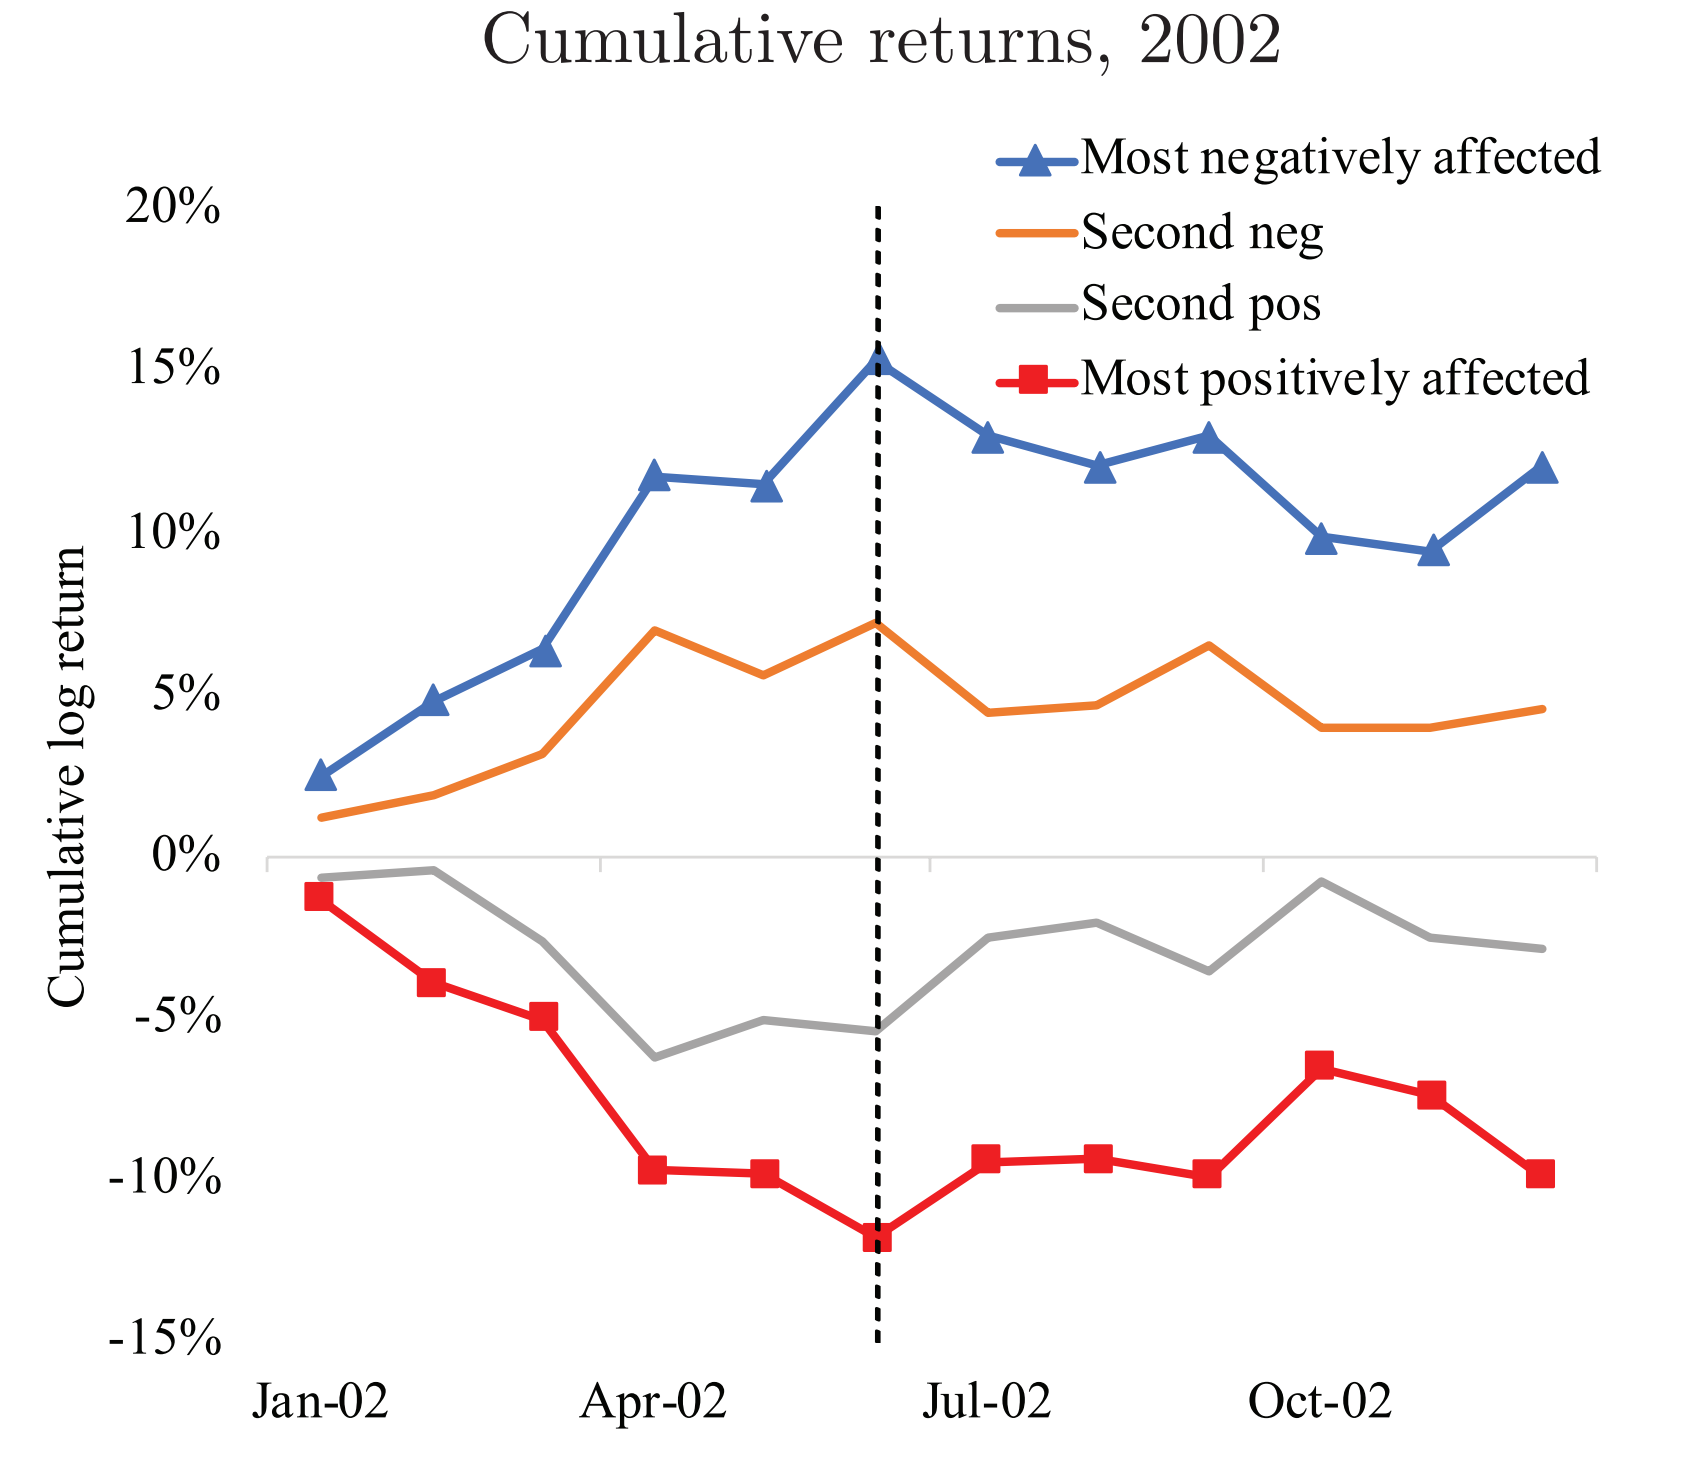
\includegraphics[width=1  \linewidth]
		    {pic/event_returns.png}
		  \end{center}
		\end{figure}
		\vspace{-0.6cm}
		\center\tiny{Cumulative style returns}
	\end{columns}
\end{frame}

\begin{frame}{Placebo test: Other years}
	\center Rerunning in all years other than 2002
	\begin{columns}
		\column{0.33\textwidth}
		\begin{figure}[htpb]
		  \begin{center}
		    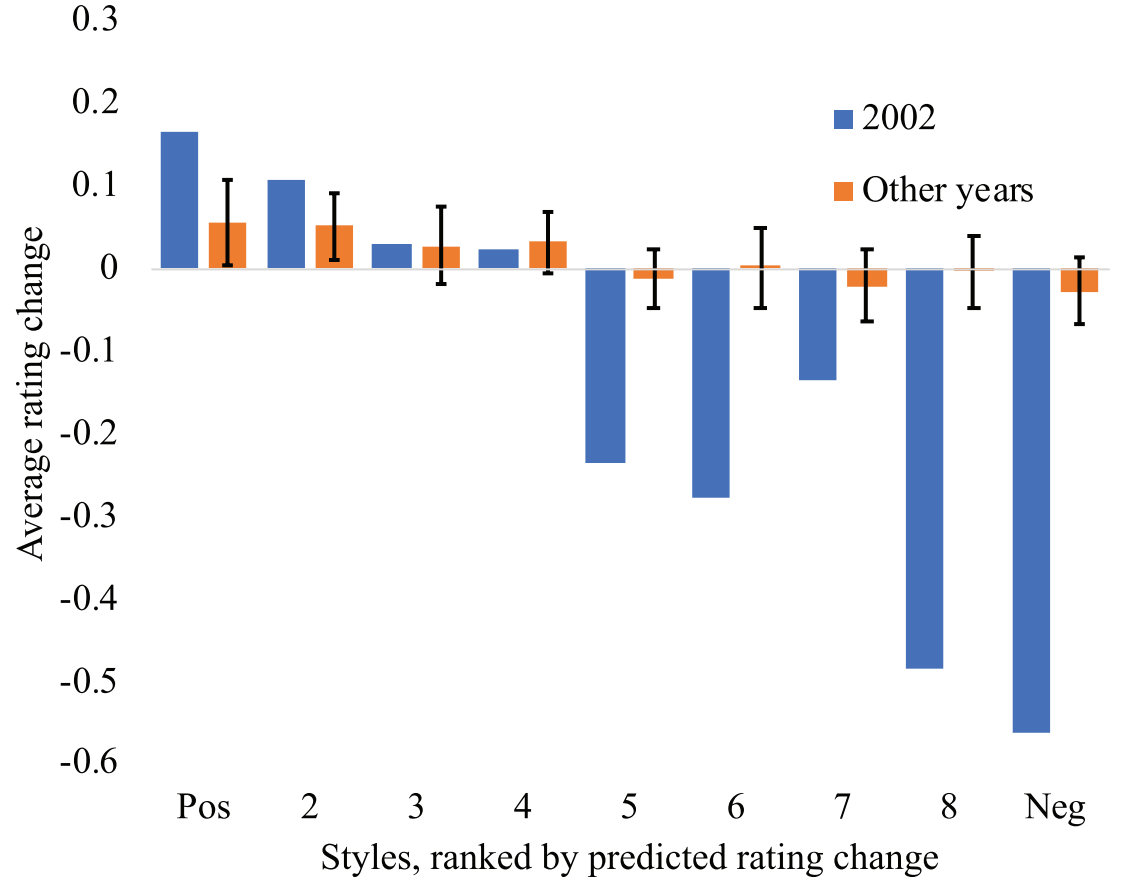
\includegraphics[width=1.1  \linewidth]
		    {pic/placebo_ratings.png}
		  \end{center}
		\end{figure}
		\vspace{-0.6cm}
		\center\tiny{Ratings change: 2002 vs. placebo}
		\column{0.33\textwidth}
		\begin{figure}[htpb]
		  \begin{center}
		    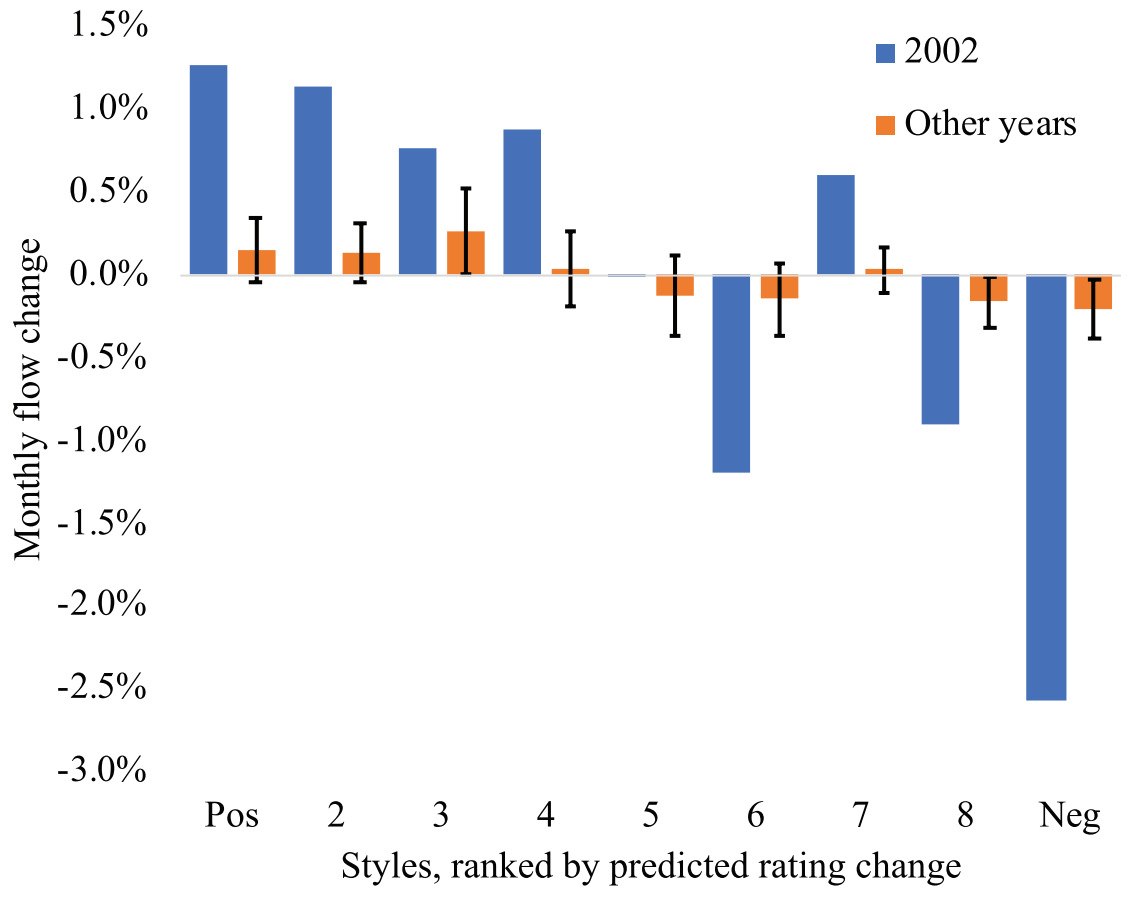
\includegraphics[width=1.1  \linewidth]
		    {pic/placebo_flows.png}
		  \end{center}
		\end{figure}
		\vspace{-0.6cm}
		\center\tiny{Flow change: 2002 vs. placebo}
		\column{0.33\textwidth}
		\begin{figure}[htpb]
		  \begin{center}
		    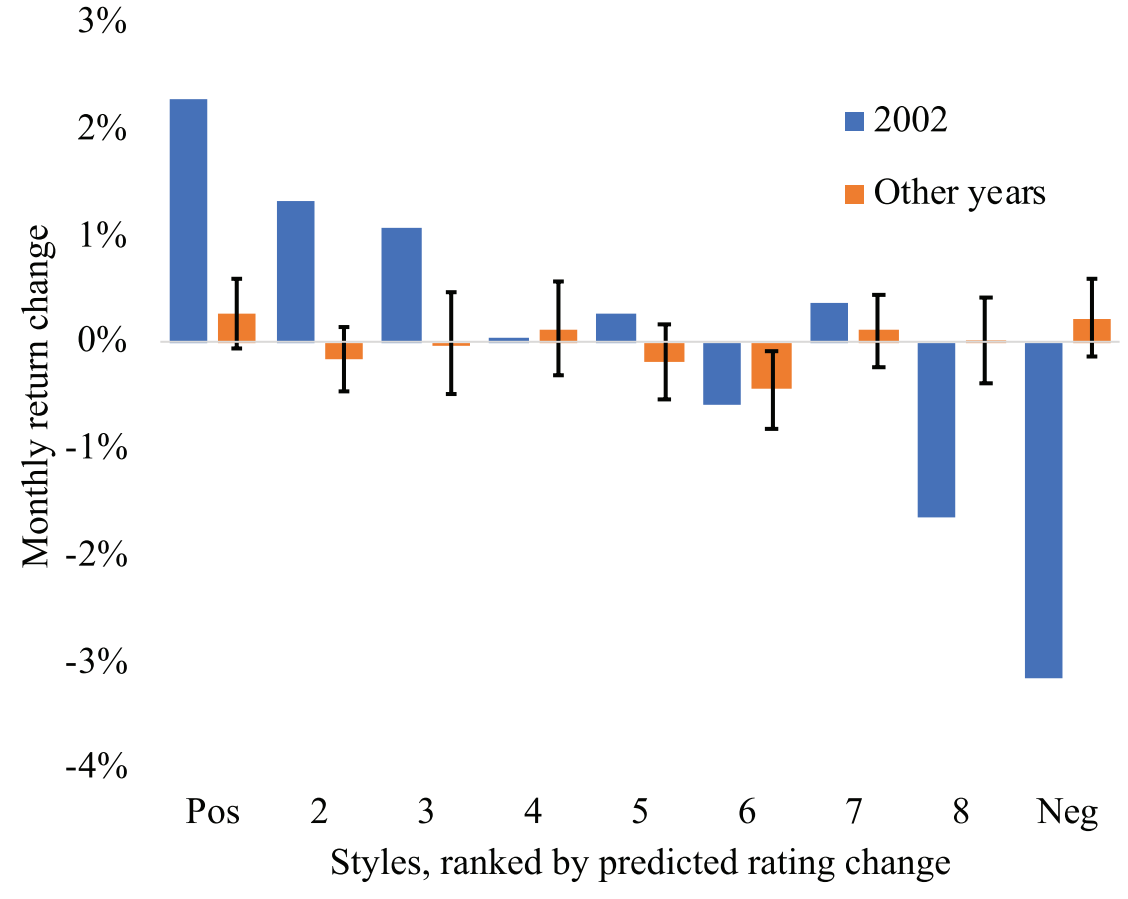
\includegraphics[width=1.1  \linewidth]
		    {pic/placebo_returns.png}
		  \end{center}
		\end{figure}
		\vspace{-0.6cm}
		\center\tiny{Return change: 2002 vs. placebo}
	\end{columns}
\end{frame}

\begin{frame}{Other factors that may have affected style returns}
	\begin{itemize}
		\item Event study methodology assumes that no other sudden style-level shocks occurred around June 2002 that could have caused the patterns
		\item The in-existence of such shocks is a key assumption that merits further validation
	\end{itemize}
	\begin{enumerate}
		\item No discernible sudden change in fundamentals (ROA and ROE) around June 2002 
		\item 13F institutions traded into (out of) styles with high (low) pre-2002 ratings, before halting suddenly right after June 2002
		\item A general slow rise in short interest across all styles over the window but no clear change around the event
	\end{enumerate}
\end{frame}

\begin{frame}{Controlling for stock characteristics}
	\begin{itemize}
		\item One might still argue that our results could be driven by sudden characteristics-related return changes that happened for other reasons
		\item \alert{``Predicted rating changes explain return changes"} also take place at the stock level after controlling for size and book-to-market ratio characteristics
		\item Even after controlling for characteristics, we should still expect to see an effect
	\end{itemize}
	
	$$
	\begin{aligned} 
	\mathrm{Rating }_{i, t}^{\text{idiosyncratic}} & =\mathrm{Rating}_{i, t}-\mathrm{Rating}_{\text{size-book/market portfolio}\ p, t}
	 \\
	  \mathrm{Ret}_{i, t}^{\text{idiosyncratic}} & =\mathrm{Ret}_{i, t}-\mathrm{Ret}_{\text {size-book/market portfolio}\ p, t}
	\end{aligned}
	$$
\end{frame}

\begin{frame}{Controlling for stock characteristics}
	\begin{figure}[htpb]
	  \begin{center}
	    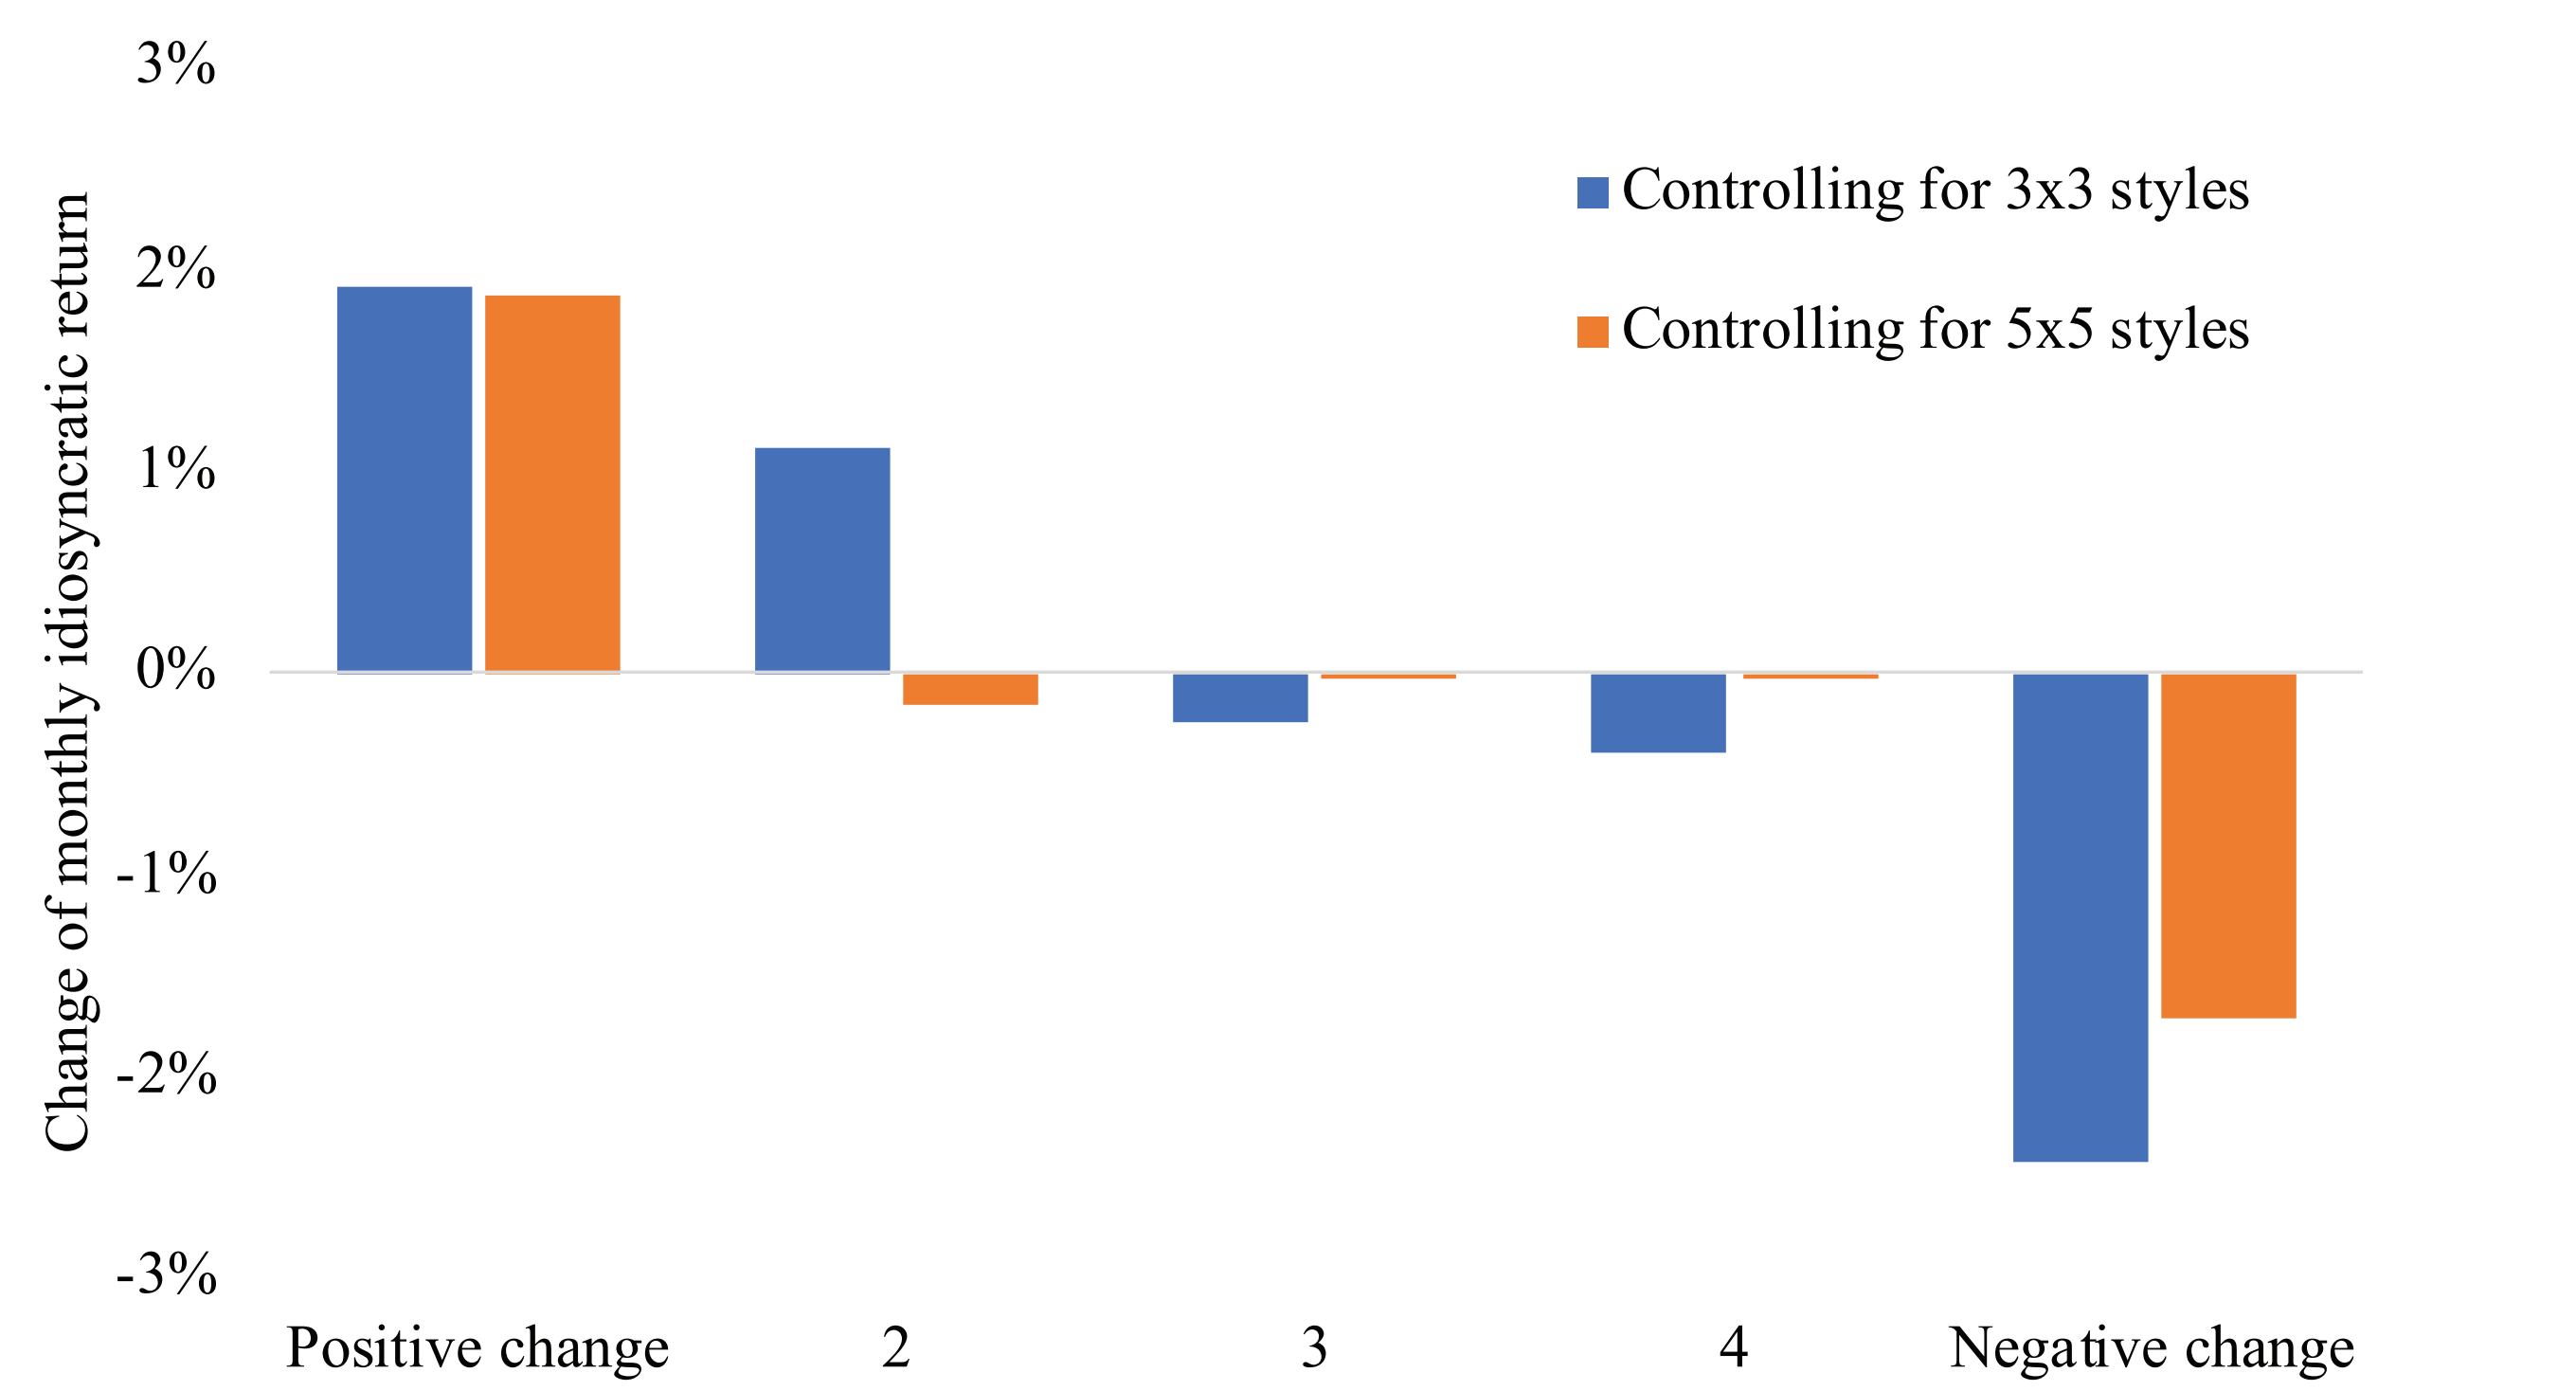
\includegraphics[width=1  \linewidth]
	    {pic/control.png}
	  \end{center}
	  \caption{Stocks sorted by predicted idiosyncratic rating}
	\end{figure}
\end{frame}

\section{Conclusion}

\begin{frame}{Conclusion}
	\begin{itemize}
		\item Morningstar rating-driven household demand for mutual funds contributes to economically significant price fluctuations at the style level
		\item These findings should alter the way economists interpret systematic price movements: instead of solely reflecting fundamental risks, they also may be determined by \alert{non-fundamental demand}
	\end{itemize}
\end{frame}

\begin{frame}{Thoughts after reading}
	\begin{itemize}
		\item Prose: the form is scattered while the spirit remains
		\item Completeness of the story
		\item More than statistical tests
		\item A new perspective of the story
	\end{itemize}
\end{frame}
%%%%%%%%%%%%%%%%%%%%%%%%%%

% End
\begin{frame}[allowframebreaks]%{End}
	\begin{center}
		\Huge\textbf{\textit{\texttt{Thanks!}}}
	\end{center}
\end{frame}

% Reference
%\appendix
%\begin{frame}{Reference}
%	\addtocounter{framenumber}{-1}
%	\printbibliography % [heading=bibintoc, title=Reference]
%\end{frame}

%%%%%%%%%%%%%%%%%%%%%%%%%%

% Snippets
%\begin{frame}[noframenumbering, plain]{Snippets}
%	\begin{multicols}{2}
%		\begin{enumerate}
%			\item \cite[Page10]{barro1990}
%			\item parencite \\ \parencite{Greiner2008}
%			\item footcite \footcite{green2020}
%			\item \cite{Greiner2008}
%		\end{enumerate}
%		\begin{itemize}
%			\item \[V = \frac{4}{3}\pi r^3\]
%			\item $ V = \frac{4}{3}\pi r^3 $
%		\end{itemize}
%	\end{multicols}	
%	\begin{equation}
%		\label{eq1}
%		V = \frac{4}{3}\pi r^3
%	\end{equation}
%	\center 
%	As Equation(\ref{eq1}) shows, $\cdots$, this \emph{equation} is \alert{important}.
%\end{frame}
%
%\begin{frame}[noframenumbering, plain]{Snippets}
%	\begin{columns}
%		\column{0.5\textwidth}
%			\begin{block}{Remark}
%				Sample text
%			\end{block}
%			\begin{alertblock}{Important theorem}
%				Sample text in red box
%			\end{alertblock}
%			\begin{examples}
%				Sample text in green box. 
%			\end{examples}
%		\column{0.5\textwidth}
%			\begin{table}
%			    \centering
%			    \caption{table1}
%			    \vspace{-0.5cm}
%			    \setlength{\tabcolsep}{5mm}
%				    {
%				    \begin{tabular}{lcc}
%				    \hline
%			        123 & 123 & ad f \\ \hline
%			        \textcolor{deepred}{123} & w & ad f \\ 
%			        \textcolor{sufered}{123} & \alert{ad} f & ad s f \\ \hline
%				    \end{tabular}
%				    }
%			    \label{fig1}
%			\end{table}
%	\end{columns}
%\end{frame}
%\backupend
%%%%%%%%%%%%%%%%%%%%%%%%%%
\end{CJK*}
\end{document}